\documentclass[12pt]{article}

\usepackage[letterpaper,margin=0.6in]{geometry}
\usepackage[T1]{fontenc}
\usepackage{microtype}
\usepackage{graphicx}
\usepackage{xcolor}
\usepackage{setspace}
\usepackage{enumitem}
\usepackage{authblk}
\usepackage{url}
\usepackage{booktabs}
\usepackage{caption}
\usepackage{subcaption}
\usepackage{csquotes}
\usepackage{array}
\usepackage{tabularx}
\usepackage{adjustbox}
\usepackage{listings}
\usepackage{newtxtext,newtxmath}
\usepackage[colorlinks=true,linkcolor=black,citecolor=black,urlcolor=minority]{hyperref}
\usepackage{float}
\usepackage{placeins}
\usepackage{titlesec}

% ---------- Colors ----------
\definecolor{majority}{HTML}{0033A0}
\definecolor{minority}{HTML}{8A8D8F}
\definecolor{black}{HTML}{000000}
\definecolor{listingbg}{HTML}{F7F7F7}

% ---------- Headers/footers ----------
\usepackage{fancyhdr}
\pagestyle{fancy}
\fancyhf{}
\renewcommand{\headrulewidth}{0.6pt}
\renewcommand{\footrulewidth}{0.6pt}
\fancyfoot[C]{\thepage}
\setlength{\headheight}{14mm}
\setlength{\headsep}{6pt}

\makeatletter
\fancypagestyle{firststyle}{
  \fancyhf{}
  \fancyhead[L]{
    
\includegraphics[height=6mm]{images/logo/nycu_logo.pdf}
  }
  \fancyhead[R]{\small \@date}
  \renewcommand{\headrulewidth}{0.6pt}
  \fancyfoot[C]{\thepage}
  \fancyfoot[L]{\footnotesize National Yang Ming Chiao Tung University}
}
\makeatother

% ---------- Title block styling ----------
\makeatletter
\renewcommand\maketitle{%
  \begin{center}
    {\LARGE\bfseries\textcolor{black}{\@title}\par}
    {\normalsize\@author \par}
  \end{center}\par
}
\makeatother

\renewcommand\Authfont{\normalsize}
\renewcommand\Affilfont{\small\normalfont}
\setlength{\affilsep}{2pt}
\setlength{\parskip}{2pt}
\setlength{\parindent}{0pt}
\captionsetup{font=small}
\captionsetup{skip=4pt}
\setlist{itemsep=2pt,topsep=2pt,parsep=0pt,partopsep=0pt}
\setlength{\textfloatsep}{10pt plus 2pt minus 2pt}
\setlength{\floatsep}{8pt plus 2pt minus 2pt}
\setlength{\intextsep}{8pt plus 2pt minus 2pt}
\setlength{\abovecaptionskip}{4pt}
\setlength{\belowcaptionskip}{2pt}
\titlespacing*{\section}{0pt}{8pt}{4pt}
\titlespacing*{\subsection}{0pt}{6pt}{3pt}
\titlespacing*{\subsubsection}{0pt}{4pt}{2pt}

% ---------- Abstract styling ----------
\renewenvironment{abstract}{
  \begin{center}\bfseries Abstract\end{center}\vspace{-4pt}
  \small
}{\par\normalsize\vspace{4pt}}

% ---------- Listings ----------
\lstset{
  basicstyle=\ttfamily\footnotesize,
  breaklines=true,
  columns=fullflexible,
  frame=single,
  backgroundcolor=\color{listingbg},
  showstringspaces=false,
  keepspaces=true
}

\lstdefinestyle{appendixcode}{
  language=Python,
  basicstyle=\ttfamily\scriptsize,
  breaklines=true,
  breakatwhitespace=false,
  breakindent=0pt,
  columns=fullflexible,
  frame=single,
  backgroundcolor=\color{listingbg},
  showstringspaces=false,
  keepspaces=true,
  numbers=left,
  numberstyle=\tiny\color{minority},
  numbersep=8pt,
  xleftmargin=2em,
  framexleftmargin=1.5em,
  tabsize=4,
  postbreak=\mbox{\textcolor{minority}{$\hookrightarrow$}\space}
}

\newcolumntype{Y}{>{\raggedright\arraybackslash}X}

\title{Artificial Intelligence Project \#3 Reinforcement Learning Report}
\author[1]{414551003 Yong-Cheng Liaw}
\affil[1]{National Yang Ming Chiao Tung University}
\date{2026.05.22}

\begin{document}
\thispagestyle{firststyle}
\vspace*{-20pt}
\maketitle
\suppressfloats[t]

\section{Research Question and Motivation}

Deep reinforcement learning can appear successful when an agent reaches a high score once, but a single peak performance does not necessarily mean that the agent has learned a policy that remains effective over time. My main motivation is that a reinforcement learning method should not only discover a good policy, but also retain it. This report studies that gap through the DQN family. The central research question is: \textbf{which components of a DQN agent are most important for learning and retaining effective behavior across tasks with very different observation and reward structures?}

To answer this question, I compare six DQN variants on Lunar Lander and Atari Freeway. Lunar Lander is a compact control task with shaped rewards, while Freeway is a sparse-reward visual Atari task where progress depends on repeated successful crossings. This contrast makes the experiments more informative than a single-task comparison, because the same algorithm may fail through unstable control in one environment and through forgetting sparse-reward behavior in the other.

Rather than focusing only on final score, I examine whether an agent reaches a useful performance threshold, whether it sustains that threshold, how much performance is lost between the best checkpoint and the final checkpoint, and what the final learned behavior looks like. In each section, I use tables, learning curves, behavior figures, and cross-task summaries to show how replay buffers, target networks, Double DQN, and Dueling DQN affect learning stability and long-term policy retention.

\section{Research Method}

\subsection{AI Assistance}

I used Codex with  GPT-5.5 as programming assistance during development. The AI tool helped produce skeleton code and suggest implementation structure. I then refined each component manually, checked the model design and training logic against the project requirements, and adjusted the experiments for the final analysis.

For the report part, I first digest the results and come up with insights, then use AI to transform my insights into figures using matplotlib. I then write descriptions of the insights and use AI to improve my grammar and wording.

\subsection{Task Selection}

I chose two tasks that expose different parts of the same DQN design. LunarLander-v3 is a compact control task from the Gymnasium Box2D suite. It uses an eight-value state vector and four discrete engine actions, so the agent must learn smooth control from a small input space. Atari Freeway is an image-based Atari task built on the Arcade Learning Environment. It uses screen observations and sparse score rewards, so the agent must learn from visual input and preserve a useful crossing policy over time \cite{brockman2016openaigym,bellemare2013arcade,gymnasium_lunarlander,gymnasium_freeway}.

This pairing gives the report a simple contrast. Lunar Lander has shaped rewards that respond to distance, speed, angle, contact, and fuel use, so failures often show up as unstable landings or inefficient engine use. Freeway gives a point only when the controlled character reaches the top of the road, so failures often show up as no progress, unsafe crossings, or a policy that stops moving upward. The same algorithm family is therefore tested in both a dense, low-dimensional setting and a sparse, visual setting.

\begin{figure}[t]
  \centering
  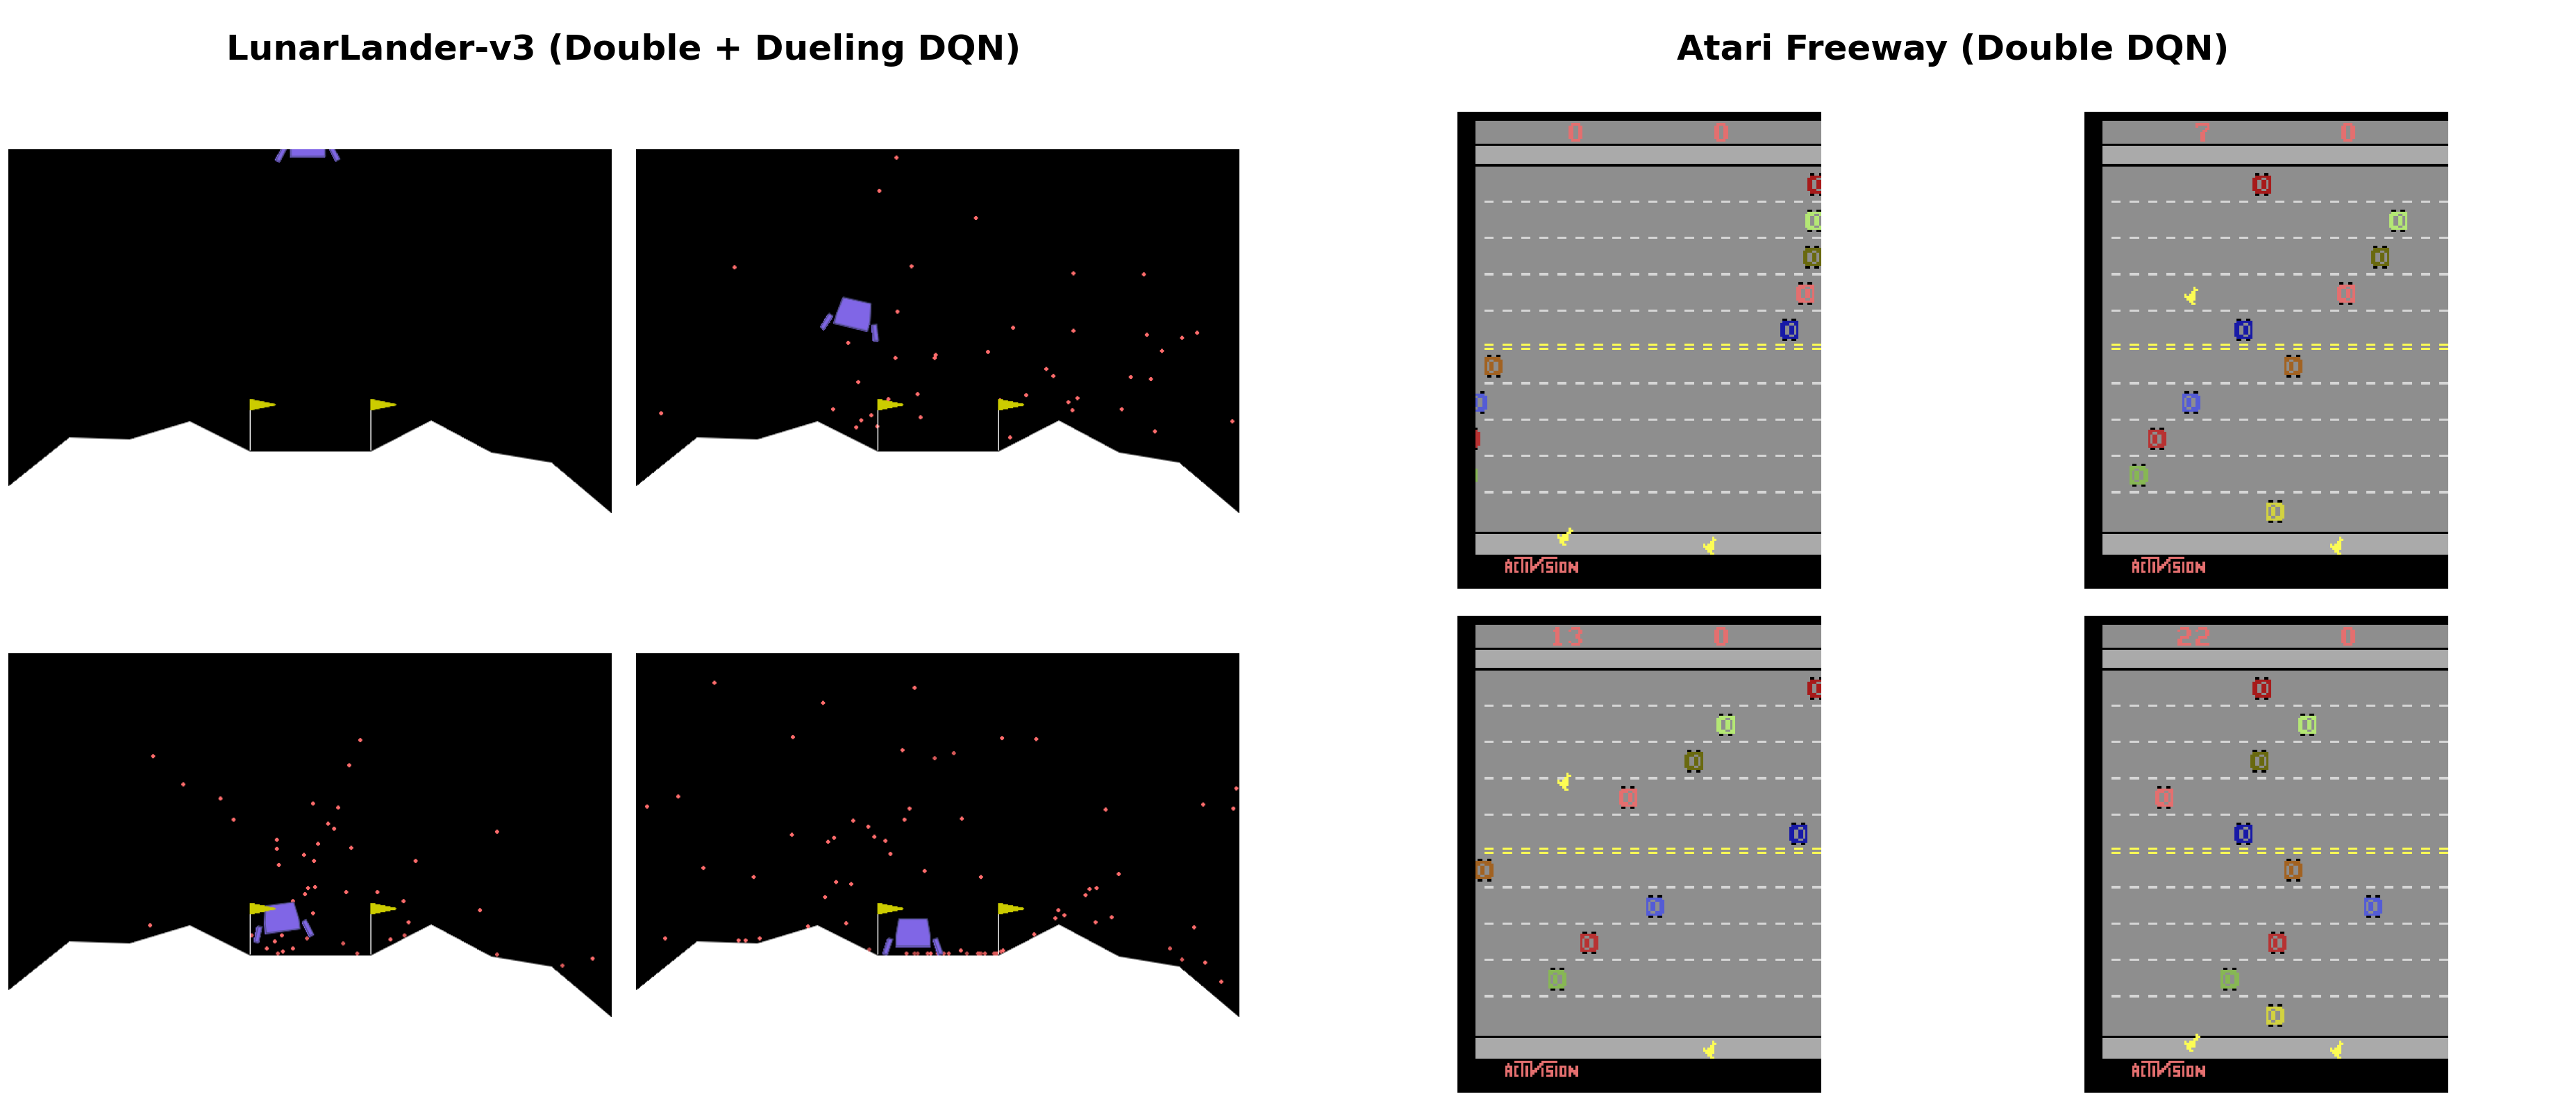
\includegraphics[width=0.8\linewidth]{helper/figures/task_selection_snapshots.png}
  \caption{Task snapshots from selected trained agents. The four snapshots on the left show the Lunar Lander agent approaching the landing zone and successfully settling on the platform between the flags. The four snapshots on the right show the Atari Freeway agent crossing traffic without being hit. In Freeway, the trained agent score is shown on the top left and the opponent score on the top right; the left score increases as the trained agent completes crossings.}
  \label{fig:task-selection-snapshots}
\end{figure}

\begin{table}[t]
  \centering
  \caption{Selected tasks for the DQN ablation study.}
  \label{tab:task-selection}
  \small
  \begin{tabularx}{\textwidth}{@{}>{\raggedright\arraybackslash}p{0.11\textwidth}>{\raggedright\arraybackslash}p{0.18\textwidth}>{\raggedright\arraybackslash}p{0.18\textwidth}>{\raggedright\arraybackslash}p{0.14\textwidth}Y@{}}
\toprule
\textbf{Task} & \textbf{Observation} & \textbf{Action Space} & \textbf{Success Signal} & \textbf{Reason for Selection} \\
\midrule
Lunar Lander & Vector state with position, velocity, angle, and leg contacts. & no-op, left engine, main engine, right engine. & Episode return at least 200. & Shaped rewards and a compact state make it useful for studying stability and sample efficiency. \\
Atari Freeway & Stacked 84 by 84 grayscale Atari frames after preprocessing. & no-op, up, down. & Score at least 15; one point is earned for each crossing. & Sparse visual rewards make it useful for testing representation learning and policy retention. \\
\bottomrule
\end{tabularx}

\end{table}

\subsection{RL Algorithm Selection and Ablation Design}

Both selected tasks have discrete action spaces, so I used the DQN family as the common algorithmic base. DQN learns an action-value function $Q(s,a)$ with a neural network and selects actions from the learned value estimates. This is a natural fit for Lunar Lander because the state is a compact vector and the action set is small. It is also a natural fit for Freeway because the original Atari DQN setting was designed for image observations and discrete joystick actions \cite{mnih2015human}.

The baseline DQN design has two important stabilizers. The replay buffer stores past transitions and samples minibatches from mixed time points, which reduces the correlation between consecutive updates and allows each useful transition to be reused. The target network is a delayed copy of the online network. It makes the Bellman target change more slowly, so the network is not always chasing a target produced by its newest parameters. The two ablations remove these mechanisms one at a time. I expected the no-replay variant to be the most fragile because it learns from recent correlated experience. I expected the no-target variant to still learn sometimes, especially in the smaller Lunar Lander state space, but to show more oscillation and weaker retention.

The remaining variants test two common DQN extensions. Double DQN uses the online network to choose the next action and the target network to evaluate that action, which is intended to reduce overestimation from the max operator \cite{vanhasselt2016deep}. Dueling DQN separates the value of a state from the relative advantage of each action, which should help when many actions have similar value in a state \cite{wang2016dueling}. The final variant combines Double DQN and Dueling DQN to test whether the two ideas are complementary rather than only useful in isolation.

\subsection{Implementation}

The project implementation uses PyTorch for the Q-networks and optimization, Gymnasium for environment interaction, and ALE through Gymnasium for Atari Freeway. The training code keeps a separate online network and, when the variant uses it, a target network. Each environment step is converted into a transition record. The replay-buffer variants store these transitions and sample minibatches with NumPy random generators, while the no-replay variants update from the newest transition only. The Double DQN variants use the online network to choose the next action and the target network to evaluate it, following the idea described in the previous subsection. The Dueling variants keep the same feature extractor but replace the single Q-value head with separate value and advantage heads. The detailed version information for the main libraries is Python 3.13.3; PyTorch 2.12.0+cu130; Gymnasium 1.3.0; NumPy 2.4.6; ALE 0.11.2;

The Lunar Lander environment is used directly as a vector-input control task. The Freeway environment uses Atari preprocessing before training: frames are converted to grayscale, resized to $84 \times 84$, repeated with frame skip, clipped by reward sign, and stacked into four-frame observations. This makes the input format close to the standard Atari DQN setting while keeping the action space small.

\subsection{Model, Training, and Experiment Settings}

\begin{figure}[htbp]
  \centering
  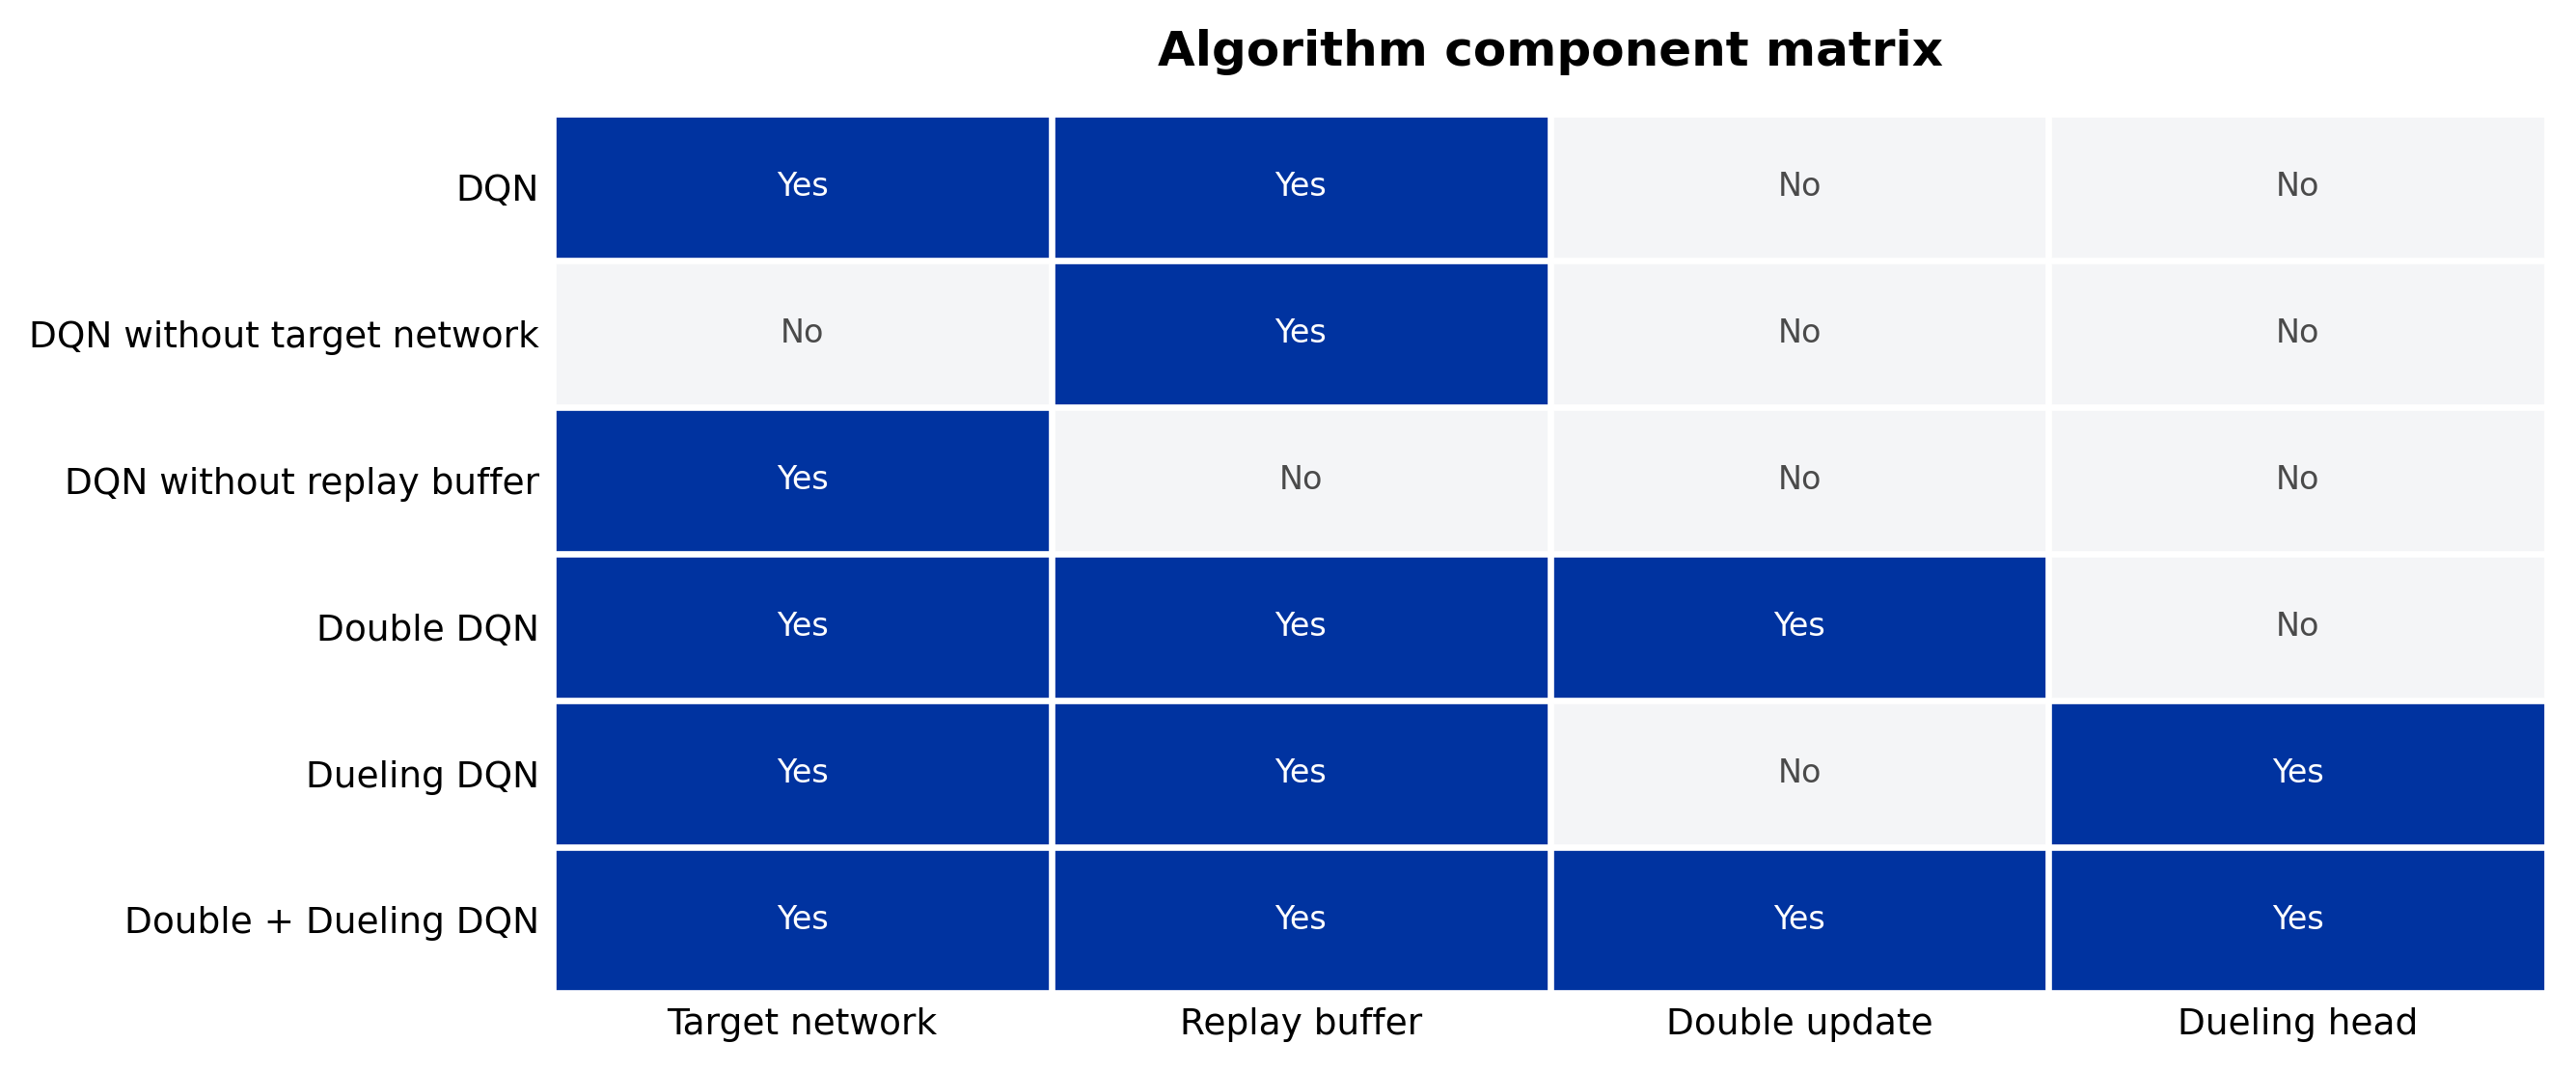
\includegraphics[width=0.9\linewidth]{helper/figures/algorithm_ablation_matrix.png}
  \caption{Component matrix for the six DQN variants.}
  \label{fig:algorithm-ablation-matrix}
\end{figure}

\begin{figure}[htbp]
  \centering
  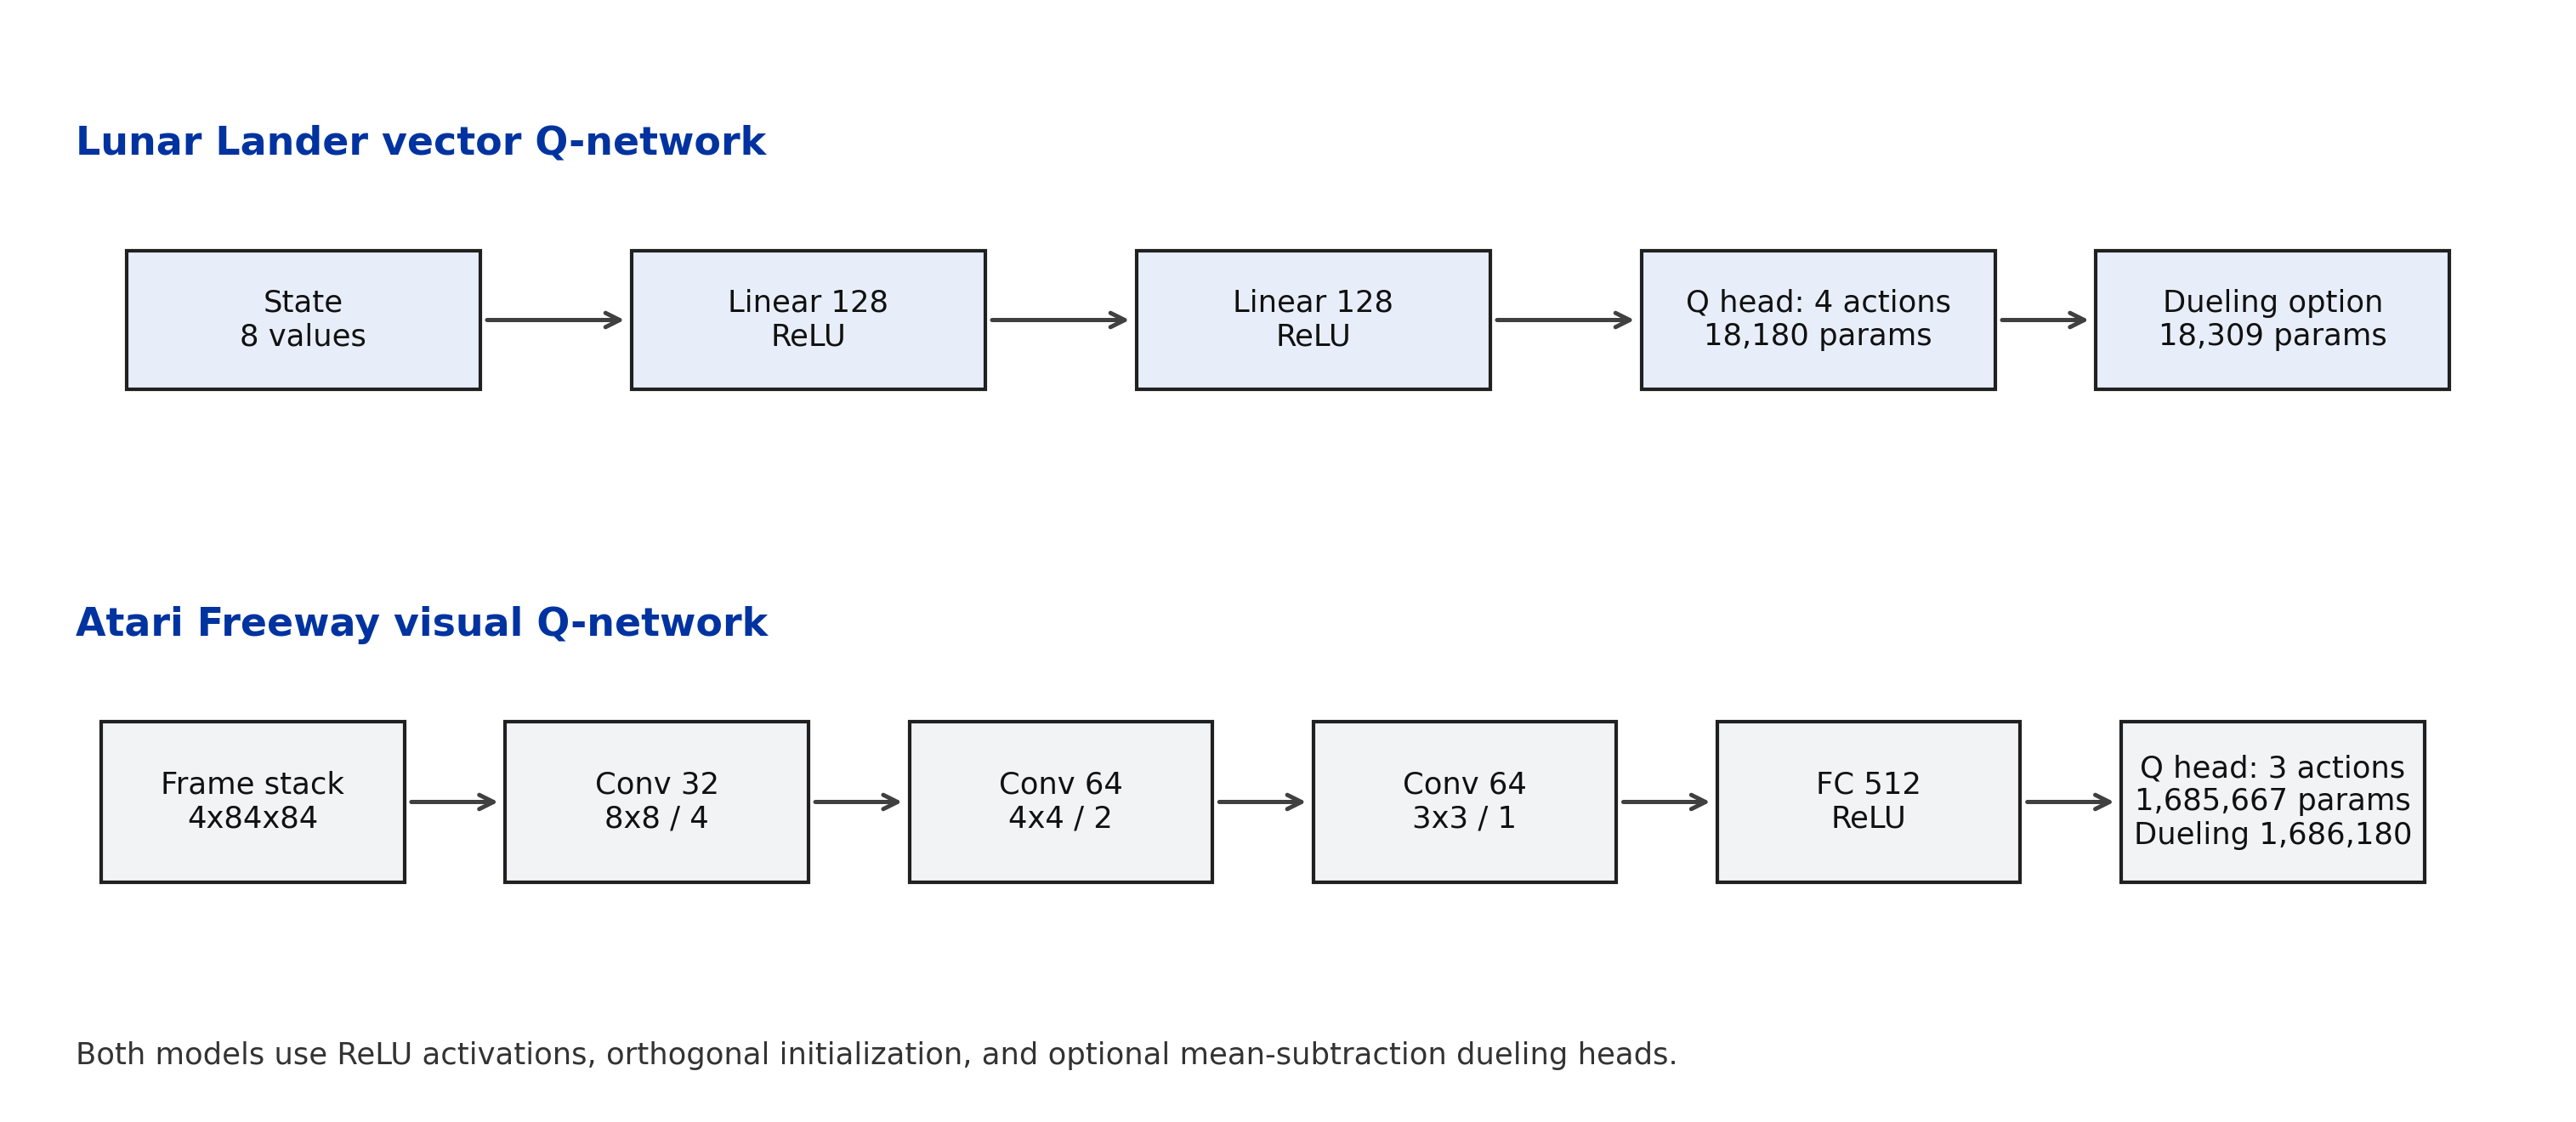
\includegraphics[width=0.9\linewidth]{helper/figures/model_architecture_overview.png}
  \caption{Network architecture overview for the vector Lunar Lander model and the visual Freeway model.}
  \label{fig:model-architecture-overview}
\end{figure}

The same six algorithm variants from Figure~\ref{fig:algorithm-ablation-matrix} were used for both tasks. Lunar Lander was run with seeds 0 through 9 for 500,000 environment steps per run. Freeway was run with seeds 0 through 3 for 1,000,000 agent steps per run, which corresponds to about 4,000,000 ALE frames because the Atari preprocessing uses frame skip 4. Evaluation used 20 episodes every 10,000 steps, and checkpoints were saved every 50,000 steps.

Figure~\ref{fig:model-architecture-overview} shows the two network families. Lunar Lander uses a small MLP because the observation is already an eight-value state vector. Freeway uses a convolutional network because the observation is a stack of image frames. For the Dueling variants, the final prediction layer is replaced by value and advantage streams with mean-subtraction aggregation. The rest of the training settings are listed in Table~\ref{tab:model-training-settings}.

\begin{table}[!htbp]
  \centering
  \caption{Model, training, and experiment settings for the selected result folders.}
  \label{tab:model-training-settings}
  \scriptsize
  \begin{tabularx}{\textwidth}{@{}>{\raggedright\arraybackslash}p{0.18\textwidth}YY@{}}
\toprule
\textbf{Setting} & \textbf{Lunar Lander} & \textbf{Atari Freeway} \\
\midrule
Variants and seeds & DQN, no-target, no-replay, Double DQN, Dueling DQN, and Double + Dueling DQN. Seeds 0-9. & DQN, no-target, no-replay, Double DQN, Dueling DQN, and Double + Dueling DQN. Seeds 0-3. \\
Training budget & 500,000 environment steps. & 1,000,000 agent steps; 4,000,000 estimated ALE frames. \\
Evaluation and checkpoints & 20 evaluation episodes every 10,000 steps; checkpoints every 50,000 steps; evaluation epsilon 0.001. & 20 evaluation episodes every 10,000 steps; checkpoints every 50,000 steps; evaluation epsilon 0.001. \\
Input preprocessing & Raw 8-value state vector; no reward clipping. & 84 by 84 grayscale frames; frame skip 4; no-op max 30; four-frame stack; clipped rewards. \\
Optimizer & Adam with learning rate 0.0005, epsilon 1e-08, weight decay 0, and gradient clipping at 10. & Adam with learning rate 6.25e-05, epsilon 0.00015, weight decay 0, and gradient clipping at 10. \\
Common DQN update & Gamma 0.99; train every 4 environment steps after 5,000 learning-start steps; 1 gradient step per update. & Gamma 0.99; train every 4 environment steps after 20,000 learning-start steps; 1 gradient step per update. \\
Replay and target defaults & Replay size 100,000; batch size 64; hard target update every 1,000 steps; target tau 1. & Replay size 25,000; batch size 32; hard target update every 8,000 steps; target tau 1. \\
No-replay override & Replay size 0; batch size 1; learning starts 0; train every 1 step. & Replay size 0; batch size 1; learning starts 0; train every 1 step. \\
Exploration schedule & Epsilon-greedy from 1 to 0.05 over 100,000 steps. & Epsilon-greedy from 1 to 0.01 over 250,000 steps. \\
\bottomrule
\end{tabularx}

\end{table}

\FloatBarrier
\section{Experiment and Discussion}

\subsection{Lunar Lander}

The Lunar Lander results show a clear separation between learning to reach the success threshold once and keeping a usable landing policy until the end of training. Table~\ref{tab:lunar-lander-summary} summarizes the six variants over ten seeds. The success reference is the same as in the method section: an evaluation return of at least 200. The table also reports whether this level was sustained over repeated evaluations, because a single high checkpoint can hide later collapse.

\begin{table}[t]
  \centering
  \caption{Lunar Lander performance, retention, and stability summary over ten seeds.}
  \label{tab:lunar-lander-summary}
  \scriptsize
  \begin{adjustbox}{width=\textwidth}
\begin{tabular}{@{}lccccccccc@{}}
\toprule
\textbf{Variant} & \textbf{Best Eval} & \textbf{Final Eval} & \textbf{Reached 200} & \textbf{Sustained 200} & \textbf{First 200} & \textbf{Final Success} & \textbf{Peak Gap} & \textbf{Largest Drop} & \textbf{Q Spike} \\
\midrule
DQN & 260.2 $\pm$ 17.3 & 208.0 $\pm$ 73.7 & 10/10 & 7/10 & 213k & 75.0\% & 52.2 & 251.2 & 10\% \\
No Target & 259.8 $\pm$ 9.4 & 149.3 $\pm$ 109.9 & 10/10 & 0/10 & 186k & 50.0\% & 110.5 & 292.2 & 100\% \\
No Replay & 127.6 $\pm$ 53.2 & -260.6 $\pm$ 215.7 & 1/10 & 0/10 & 80k & 1.5\% & 388.2 & 143.3 & 80\% \\
Double DQN & 267.2 $\pm$ 5.2 & 219.7 $\pm$ 51.7 & 10/10 & 5/10 & 261k & 74.0\% & 47.6 & 224.1 & 20\% \\
Dueling DQN & 268.3 $\pm$ 10.1 & 205.5 $\pm$ 68.4 & 10/10 & 6/10 & 255k & 69.0\% & 62.8 & 261.4 & 40\% \\
Double + Dueling & 258.3 $\pm$ 34.3 & 219.8 $\pm$ 79.7 & 9/10 & 9/10 & 261k & 77.5\% & 38.4 & 187.6 & 40\% \\
\bottomrule
\end{tabular}
\end{adjustbox}

\end{table}

\subsubsection{Learning Curves}

Figure~\ref{fig:lunar-lander-learning-curves} shows that the replay-buffer variants all learn useful policies, but they do not improve in exactly the same way. The baseline DQN reaches the 200 return threshold earlier on average than the Double and Dueling variants, with a mean first-threshold step of 213k. However, its final mean return is 208.0, below the best final variants. Double DQN and Double + Dueling DQN end at almost the same final mean return, 219.7 and 219.8. This suggests that the larger final gain comes more from stable value updates than from faster early learning.

The no-replay ablation is the main failure case. It has some early positive movement, but the mean curve drops far below the other variants and ends at -260.6. This supports the expectation from the ablation design: for Lunar Lander, recent correlated transitions are not enough to keep a reliable value function, even though the state space is small.

\begin{figure}[t]
  \centering
  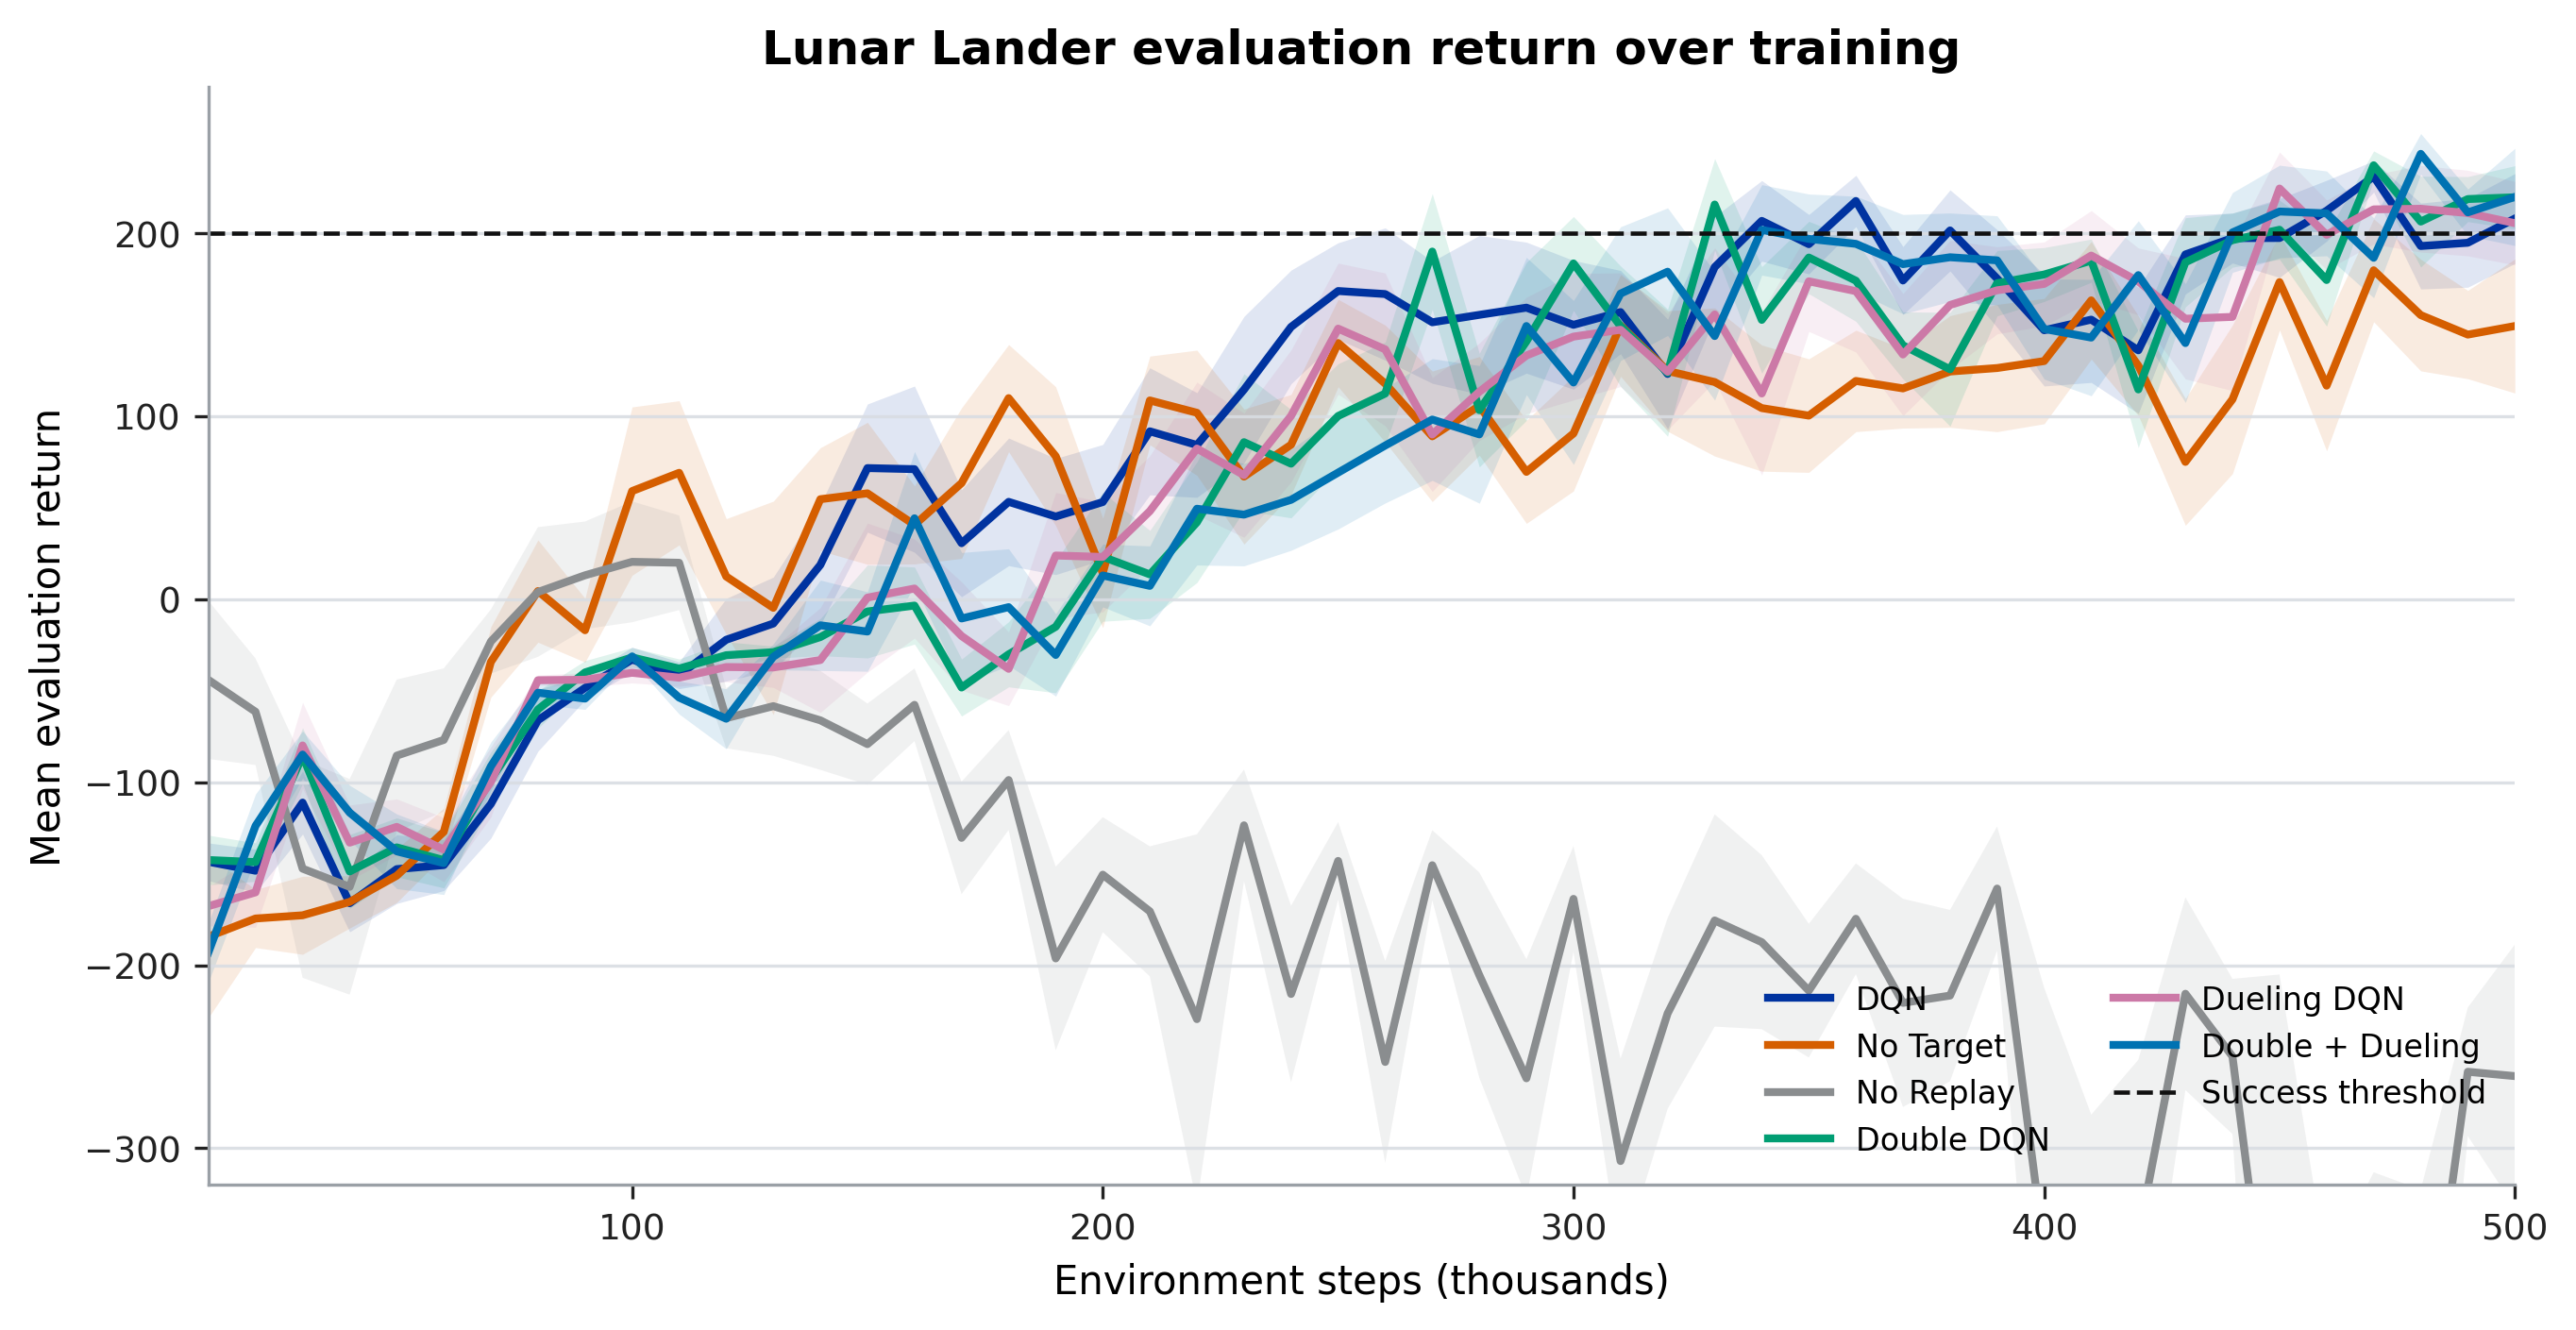
\includegraphics[width=0.92\linewidth]{helper/figures/lunar_lander_learning_curves.png}
  \caption{Mean Lunar Lander evaluation return over ten seeds. Shaded bands show the standard error across seeds, and the dashed line marks the return-200 success threshold.}
  \label{fig:lunar-lander-learning-curves}
\end{figure}

\subsubsection{Final Behavior}

\begin{figure}[H]
  \centering
  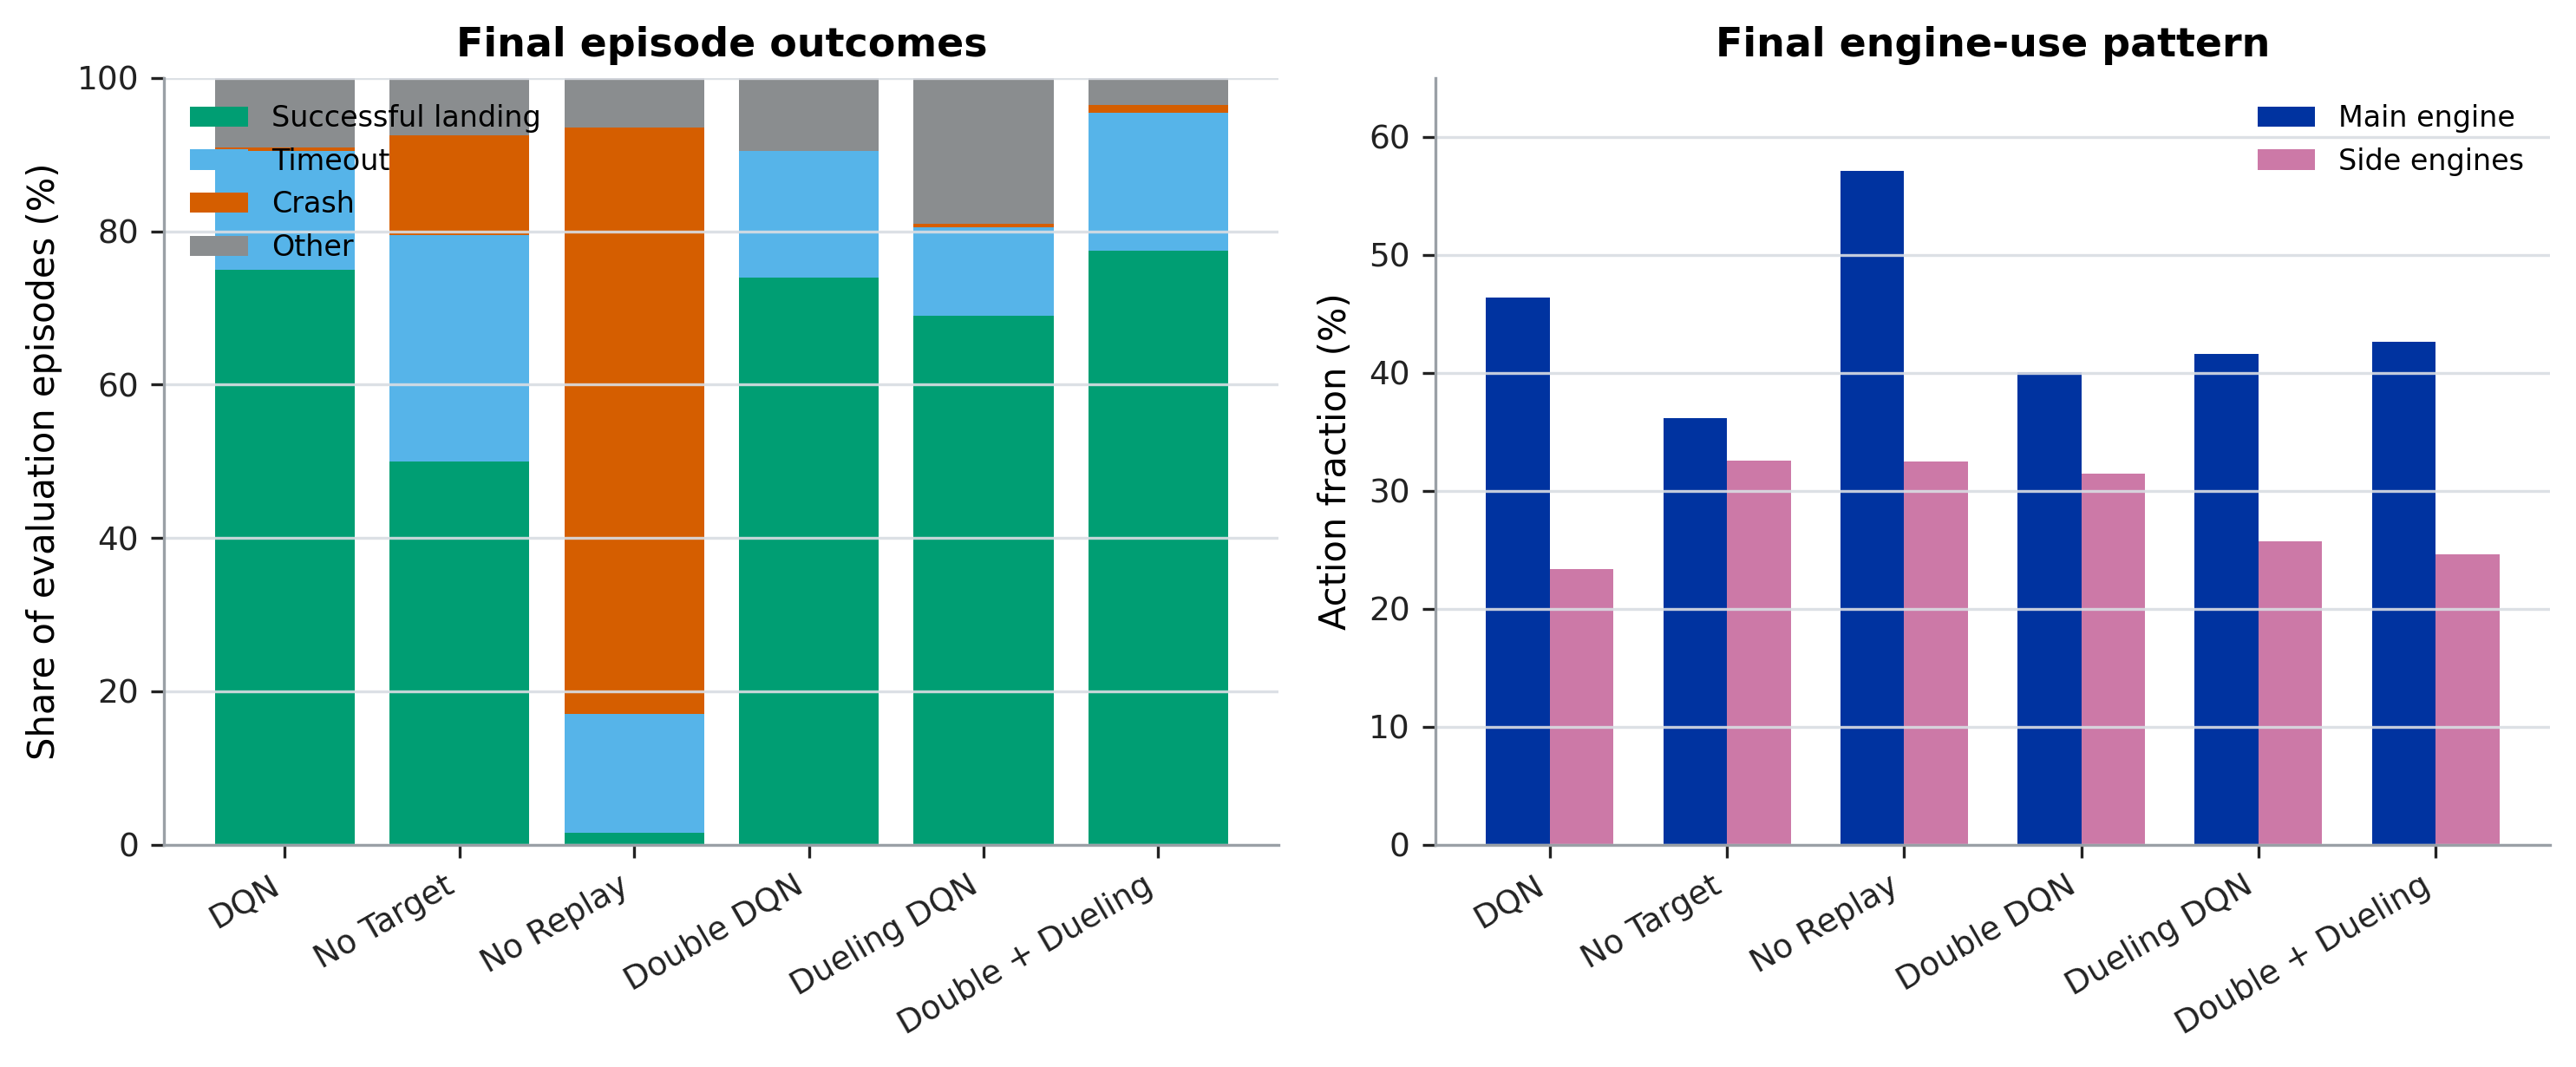
\includegraphics[width=0.9\linewidth]{helper/figures/lunar_lander_behavior_breakdown.png}
  \caption{Final Lunar Lander behavior. The left panel compares episode outcomes, and the right panel compares final engine-use fractions.}
  \label{fig:lunar-lander-behavior}
\end{figure}

Figure~\ref{fig:lunar-lander-behavior} gives a more concrete view of what the final returns mean. The stronger variants mostly shift from timeout-heavy hovering to completed landings. Double + Dueling DQN has the highest final landing success rate at 77.5\%, followed by DQN at 75.0\% and Double DQN at 74.0\%. The no-replay variant instead crashes in 76.5\% of final evaluation episodes and succeeds in only 1.5\%, which explains why its final return is much lower than the others.

The action pattern also changes with better policies. The no-replay policy uses the main engine in 57.1\% of final actions, much more than the successful variants. This looks like inefficient vertical control rather than a controlled landing strategy. Double DQN uses the side engines more than the other strong variants, while Double + Dueling DQN gets the best landing rate with a lower side-engine fraction. This suggests that the combined variant does not merely fire more engines; it uses the compact state information more selectively near the landing pad.

\subsubsection{Policy Retention}

The retention results are the most important extra insight from Lunar Lander. The no-target variant reaches return 200 in all ten seeds and reaches it earlier than the other variants on average, but it sustains the threshold in zero seeds. Its mean peak-to-final gap is 110.5, and its mean largest evaluation drop is 292.2. In plain terms, it can discover a good landing policy, but the policy is not held reliably as training continues.

\begin{figure}[H]
  \centering
  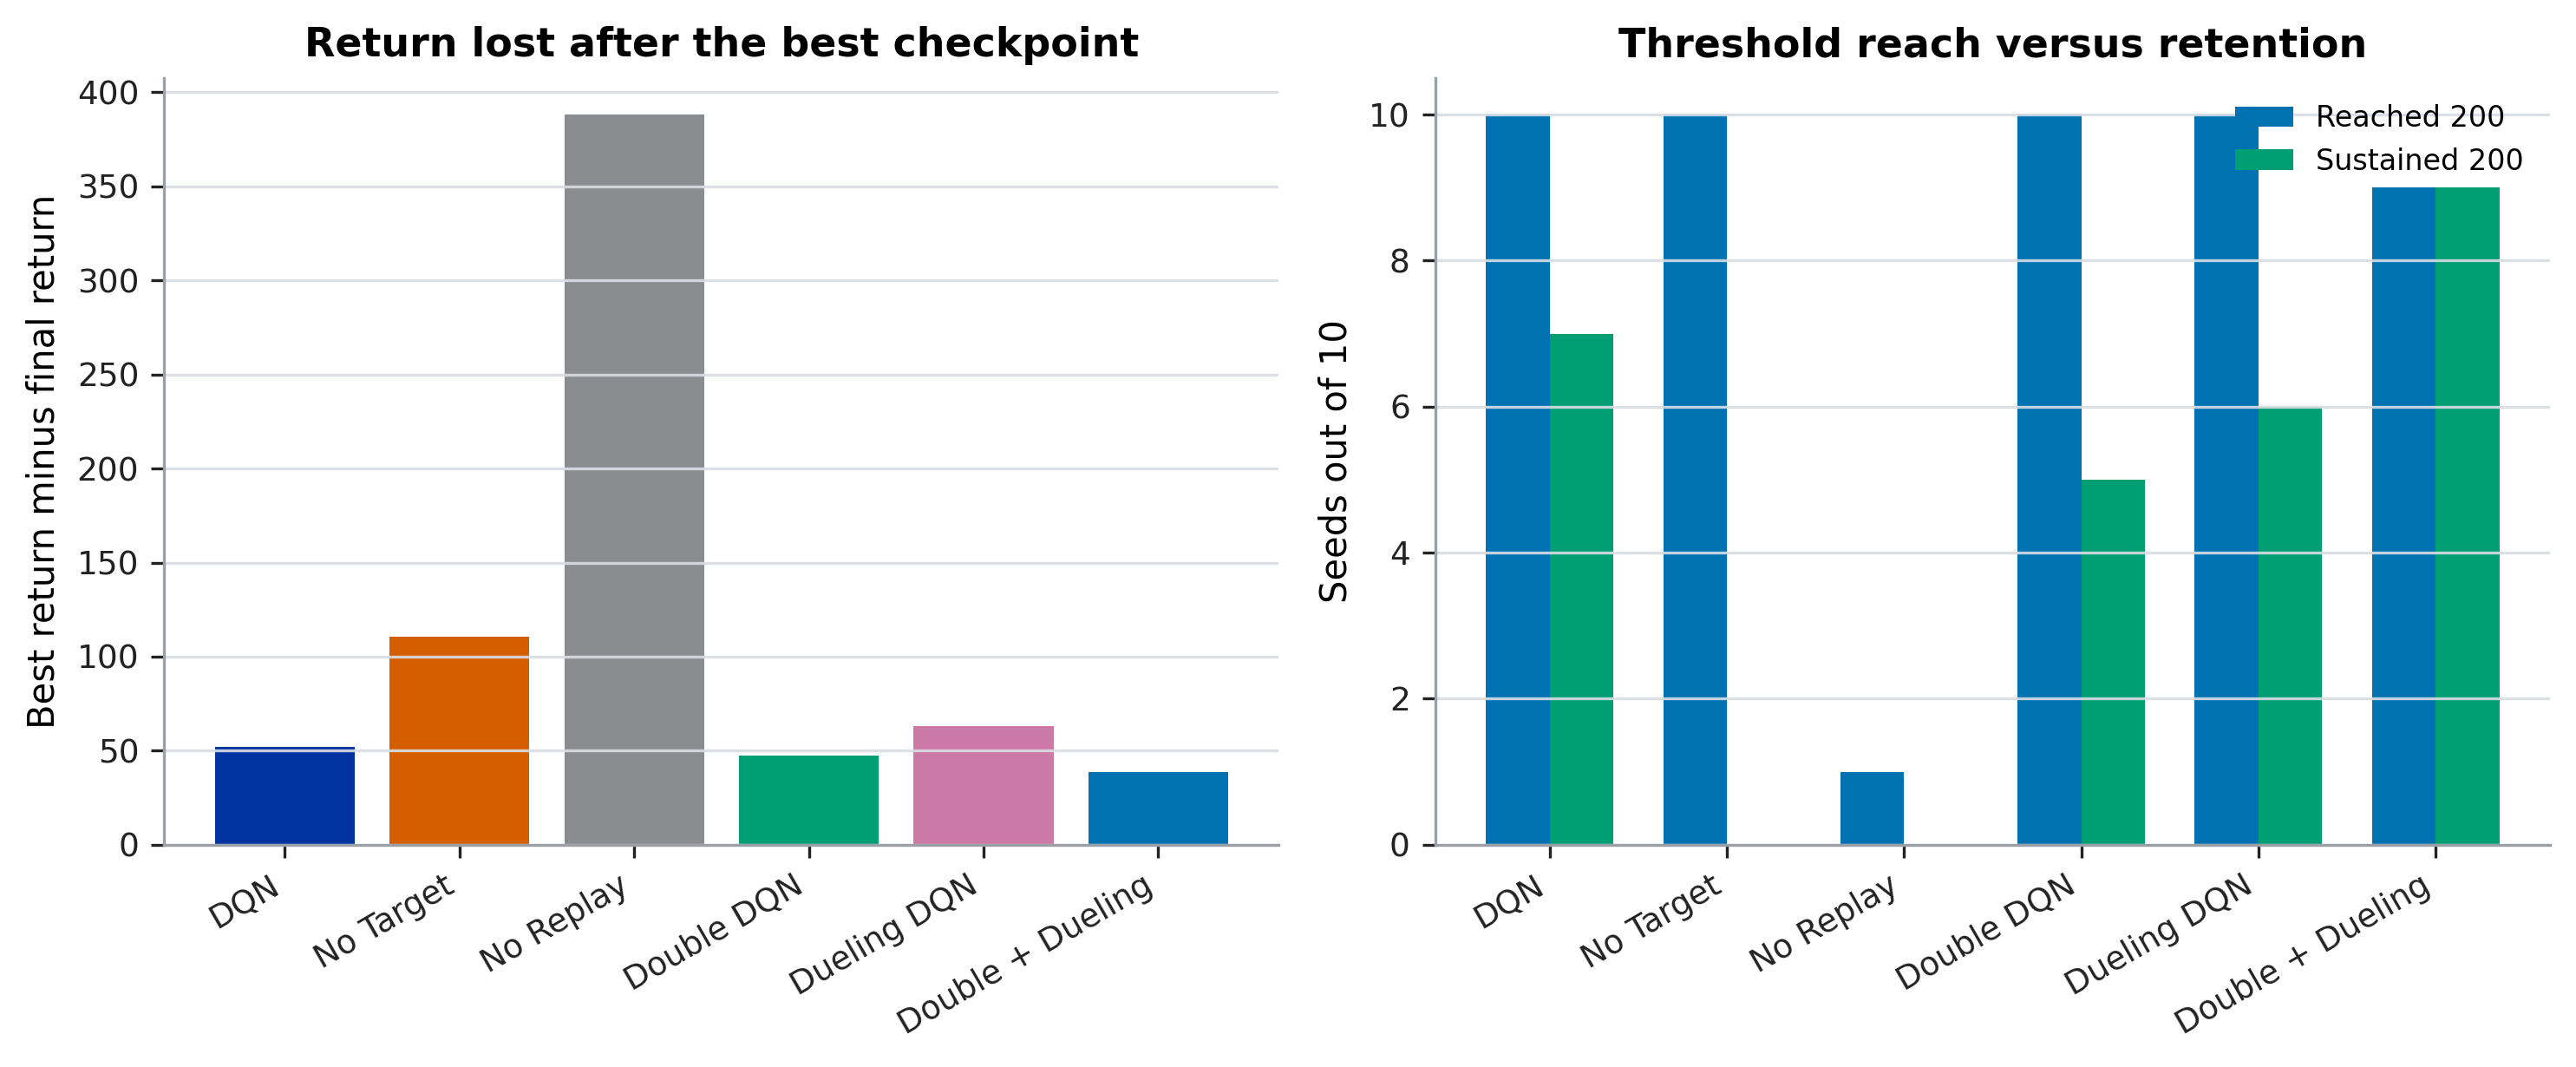
\includegraphics[width=0.9\linewidth]{helper/figures/lunar_lander_retention_gap.png}
  \caption{Policy retention after learning. The left panel shows the average drop from each seed's best evaluation return to its final evaluation return. The right panel compares seeds that reached the threshold with seeds that sustained it.}
  \label{fig:lunar-lander-retention}
\end{figure}

Double + Dueling DQN shows the opposite pattern. It reaches the threshold in nine seeds rather than all ten, but it also sustains the threshold in nine seeds and has the smallest peak-to-final gap among the high-performing variants, 38.4. Double DQN has the lowest final-return standard deviation among the best final performers, 51.7, so it is the more consistent final-return choice. The combined variant is better when the main concern is holding a successful policy once it appears.

\subsubsection{Optimization Stress}

Figure~\ref{fig:lunar-lander-optimization-stress} explains why the two ablations fail in different ways. The no-replay variant has a much larger value scale than the others, with a mean maximum Q value around 2443.8 and a final TD error around 2.12. This is consistent with unstable bootstrapping from narrow recent experience. The no-target variant has a smaller value scale, but it has a 100\% large-Q-spike rate and the highest mean collapse count, 18.8. This matches the retention result: without a delayed target network, learning can make progress, but the target changes too quickly for the policy to stay stable.

Overall, Lunar Lander confirms that replay is essential for this implementation, while the target network is essential for keeping good behavior after it is found. The best final choices are Double DQN and Double + Dueling DQN. Double DQN is the steadier final-return option, and Double + Dueling DQN is the stronger retention option.

\begin{figure}[t]
  \centering
  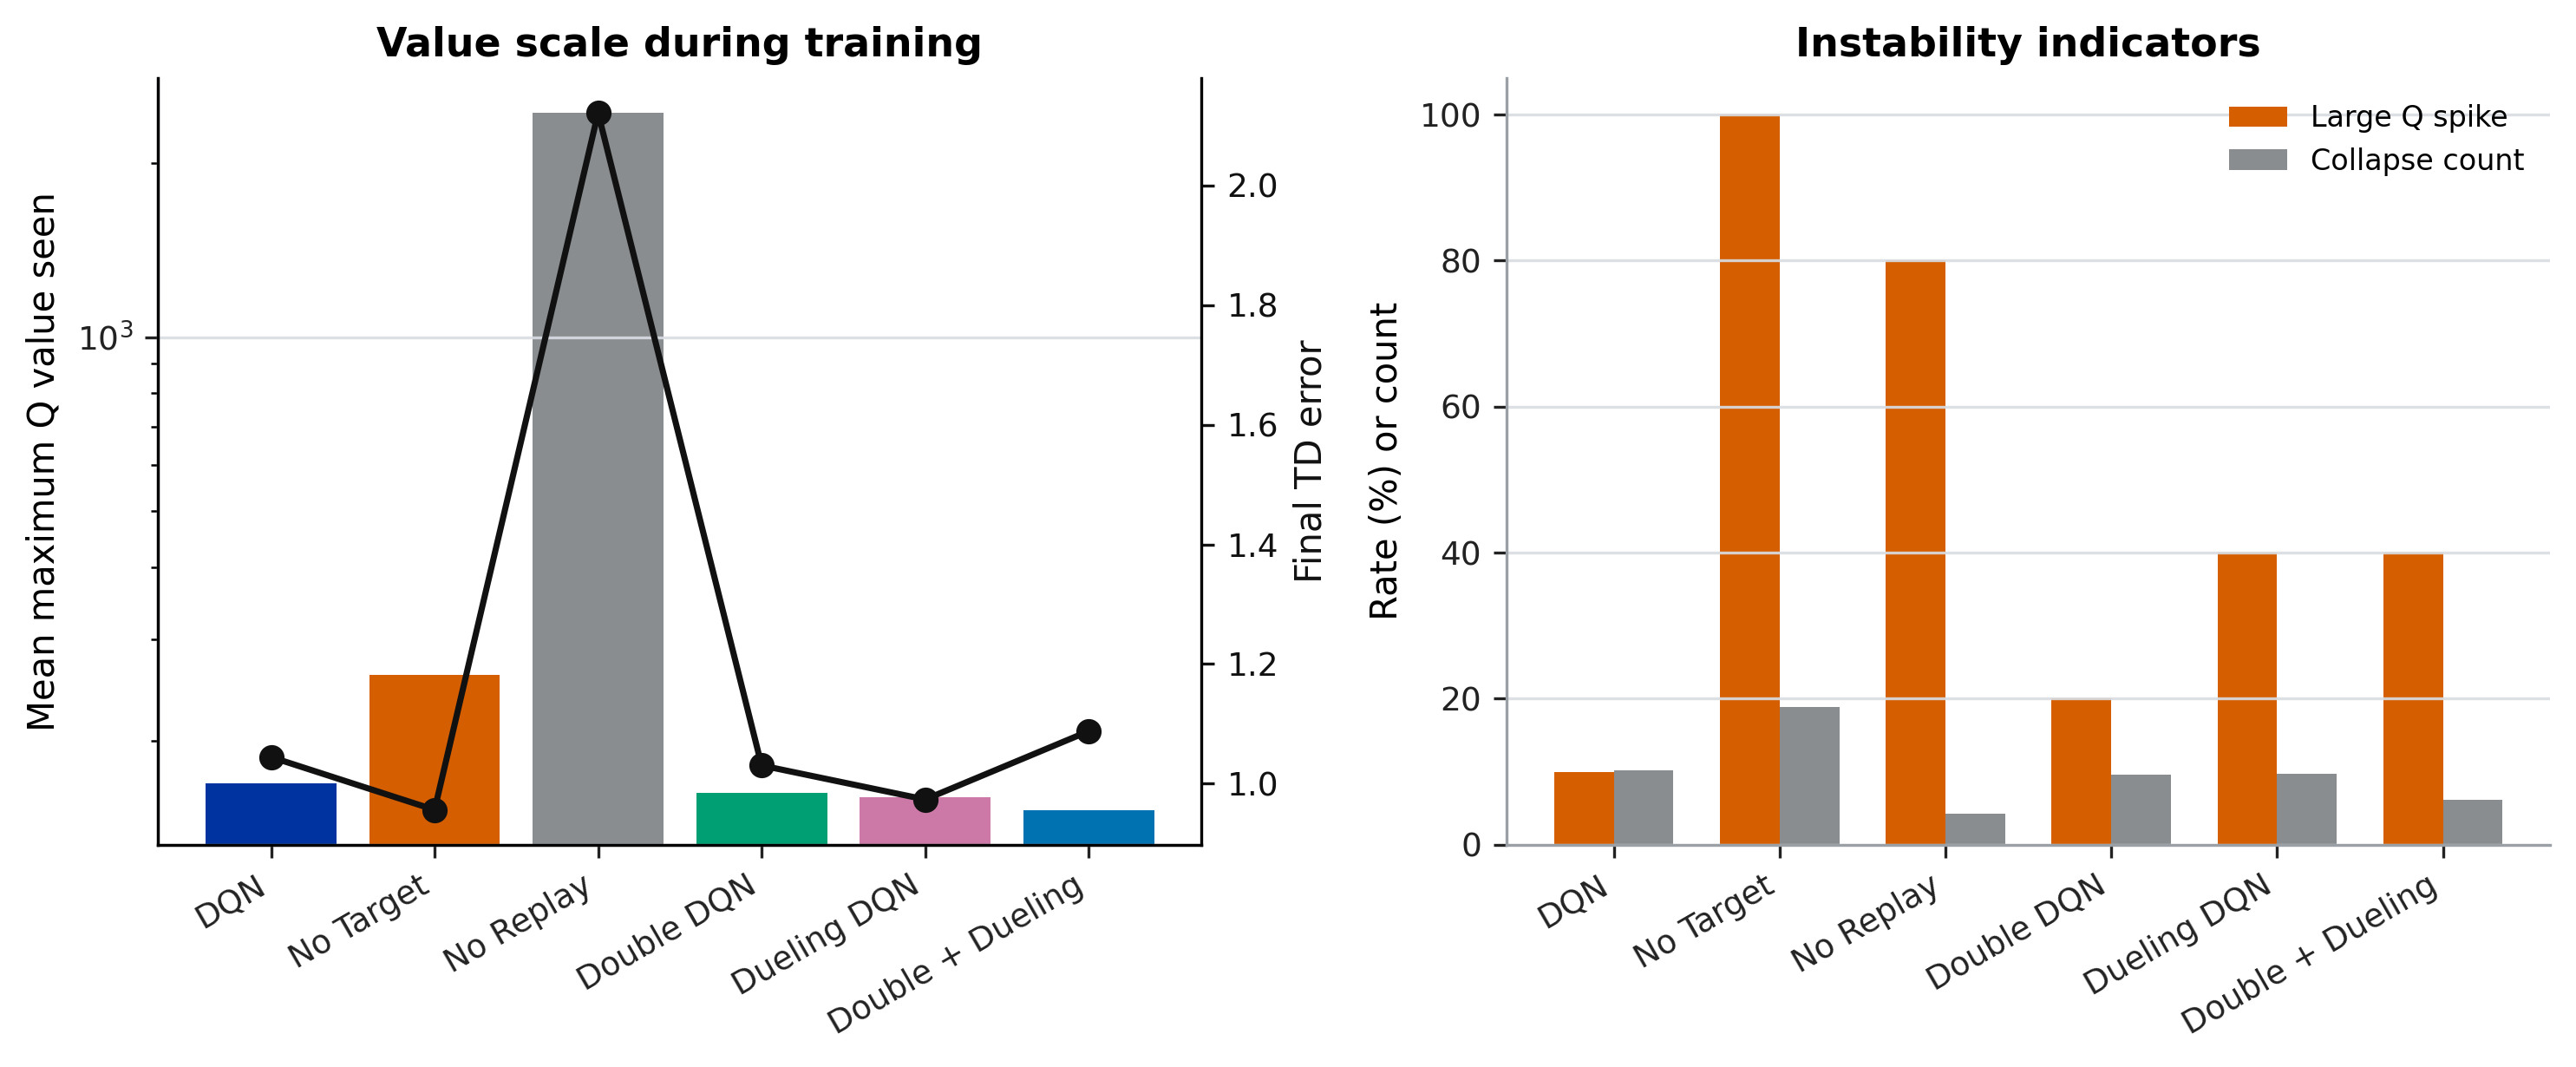
\includegraphics[width=0.85\linewidth]{helper/figures/lunar_lander_optimization_stress.png}
  \caption{Optimization stress indicators for Lunar Lander. The value-scale panel uses a log axis for maximum Q values and overlays final TD error. The instability panel compares large-Q-spike rate with average collapse count.}
  \label{fig:lunar-lander-optimization-stress}
\end{figure}

\subsection{Atari Freeway}

The Atari Freeway results test the same DQN variants in a sparse visual task. Table~\ref{tab:freeway-summary} summarizes the six variants over four seeds. The main success reference is a score of at least 15, as in the task-selection table. I also report whether each variant reaches score 22.5, because this separates basic crossing behavior from policies that are closer to the strong final scores.

\begin{table}[!htbp]
  \centering
  \caption{Atari Freeway performance, retention, and final behavior summary over four seeds.}
  \label{tab:freeway-summary}
  \scriptsize
  \begin{adjustbox}{width=\textwidth}
\begin{tabular}{@{}lccccccccc@{}}
\toprule
\textbf{Variant} & \textbf{Best Eval} & \textbf{Final Eval} & \textbf{Reached 15} & \textbf{Sustained 15} & \textbf{First 15} & \textbf{Reached 22.5} & \textbf{Final Zero} & \textbf{Up Action} & \textbf{Peak Gap} \\
\midrule
DQN & 29.1 $\pm$ 0.8 & 28.3 $\pm$ 0.7 & 4/4 & 4/4 & 198k & 4/4 & 0.0\% & 79.8\% & 0.8 \\
No Target & 29.3 $\pm$ 0.3 & 27.2 $\pm$ 1.2 & 4/4 & 4/4 & 55k & 4/4 & 0.0\% & 76.2\% & 2.1 \\
No Replay & 21.6 $\pm$ 2.8 & 5.8 $\pm$ 9.7 & 4/4 & 1/4 & 32k & 2/4 & 56.2\% & 30.0\% & 15.7 \\
Double DQN & 29.7 $\pm$ 0.9 & 29.3 $\pm$ 1.1 & 4/4 & 4/4 & 238k & 4/4 & 0.0\% & 80.0\% & 0.4 \\
Dueling DQN & 29.7 $\pm$ 0.5 & 28.9 $\pm$ 0.8 & 4/4 & 4/4 & 245k & 4/4 & 0.0\% & 77.9\% & 0.8 \\
Double + Dueling & 29.2 $\pm$ 0.2 & 28.3 $\pm$ 0.8 & 4/4 & 4/4 & 145k & 4/4 & 0.0\% & 79.4\% & 0.9 \\
\bottomrule
\end{tabular}
\end{adjustbox}

\end{table}

\begin{figure}[H]
  \centering
  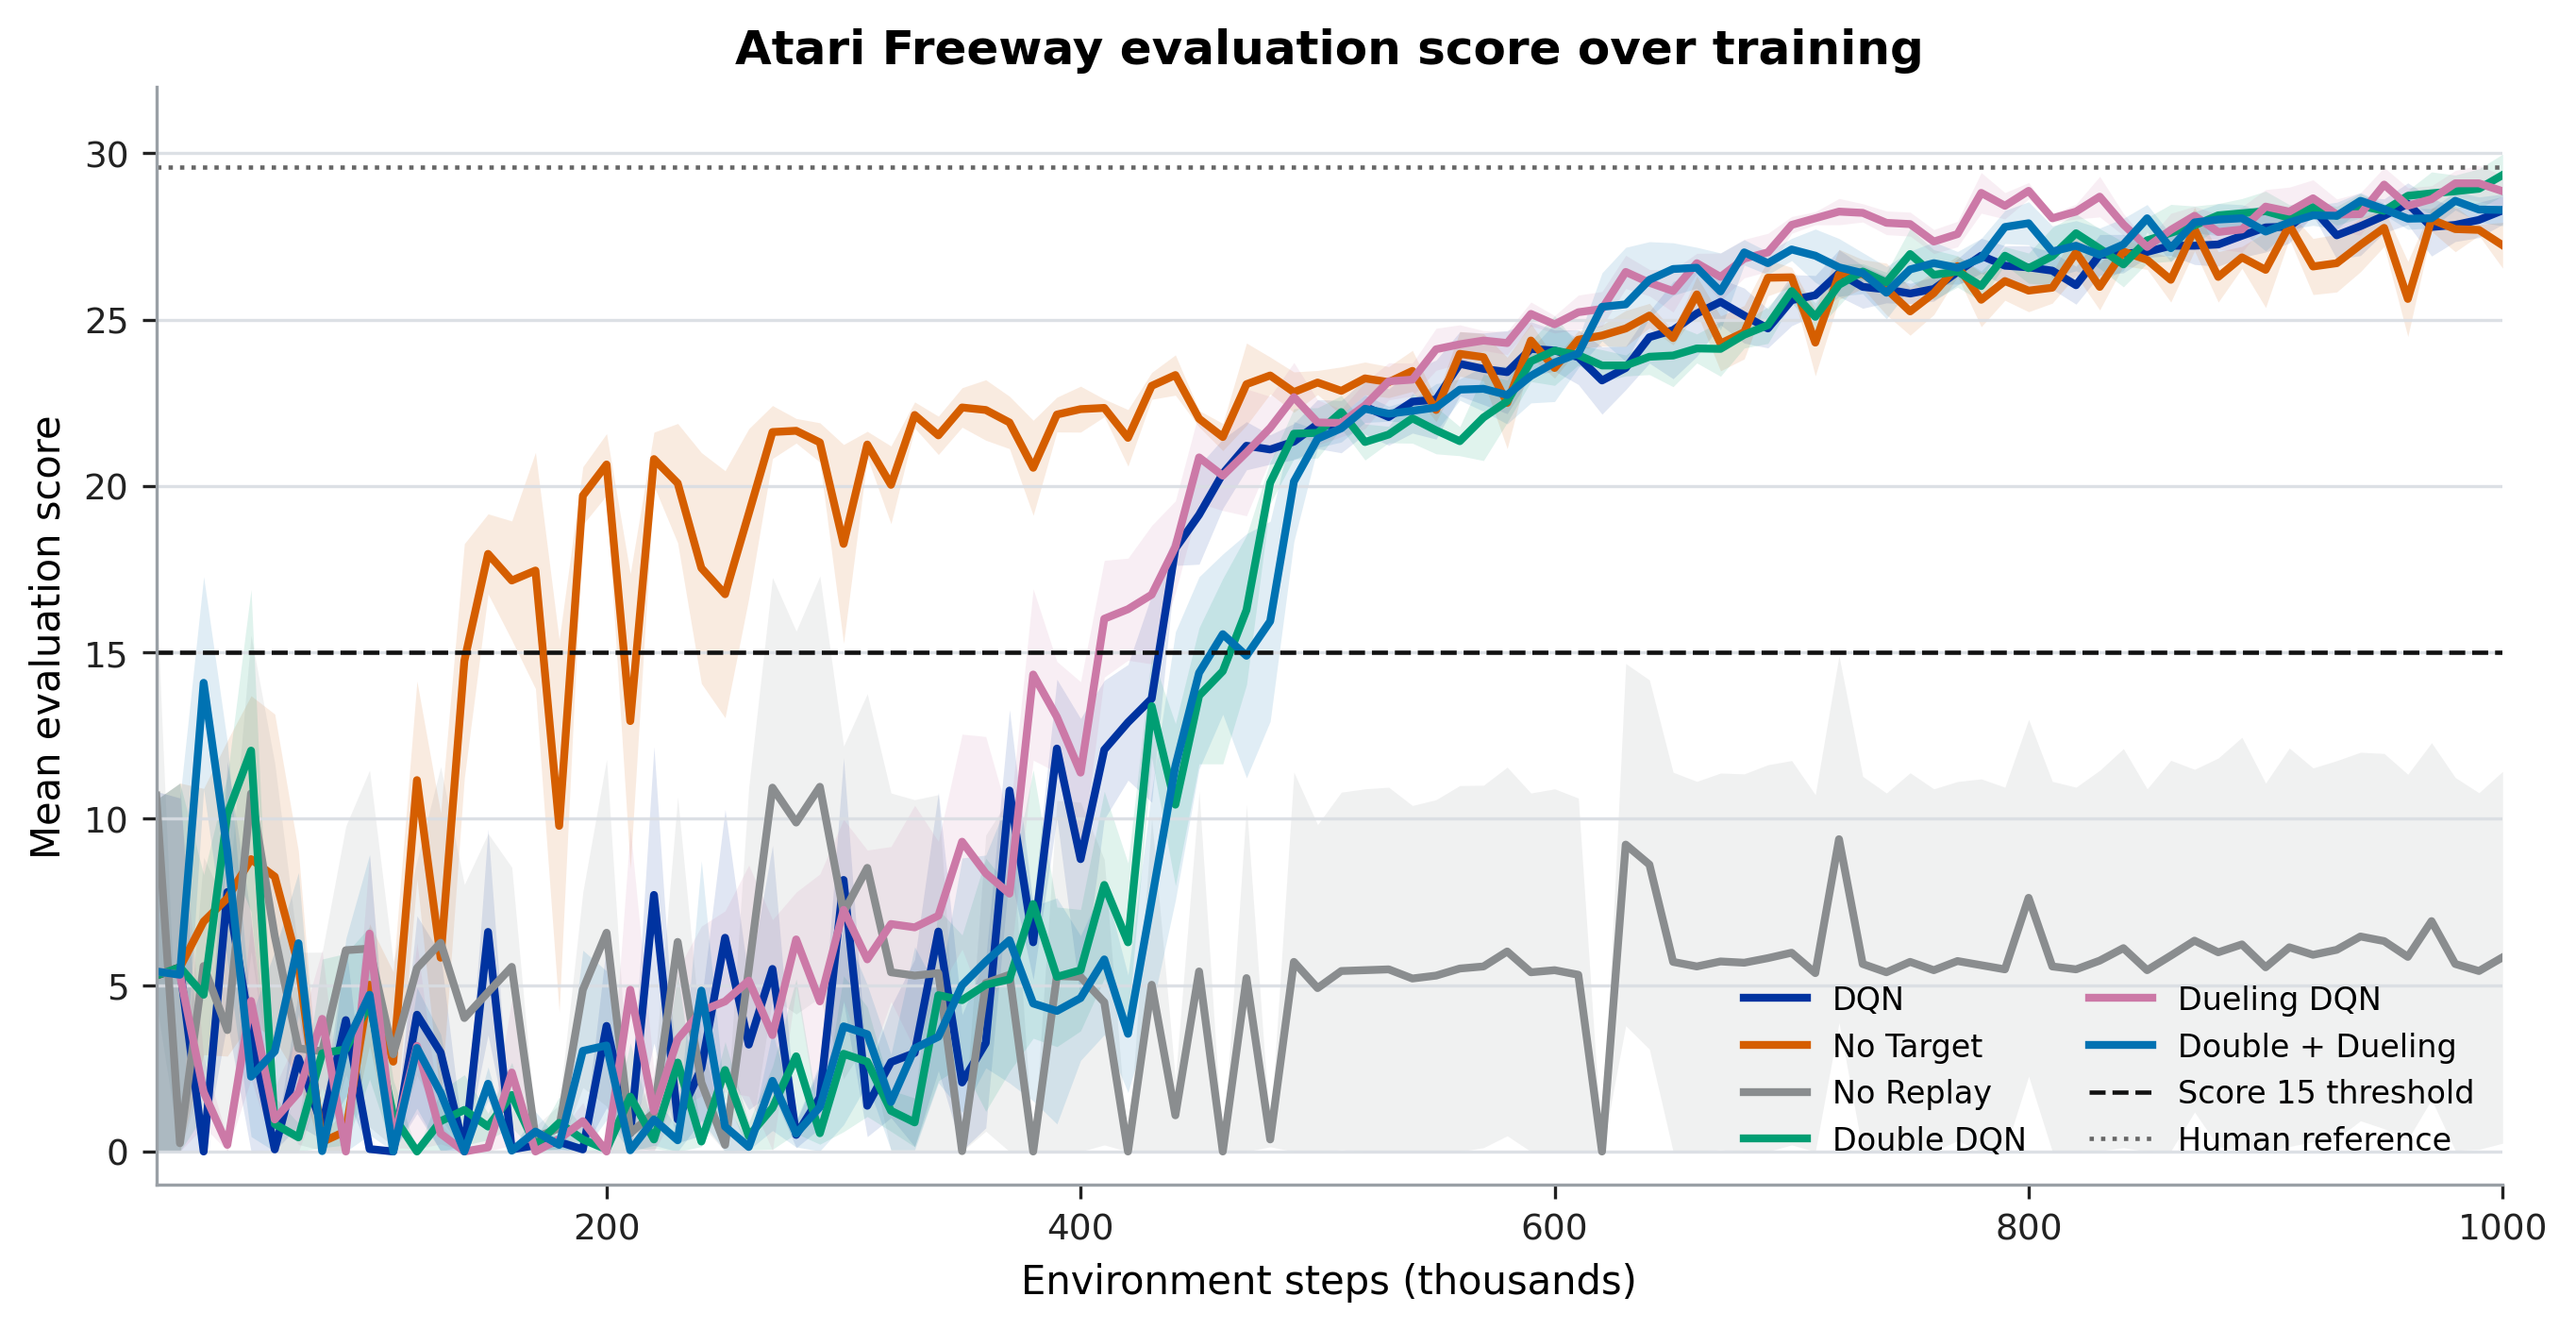
\includegraphics[width=0.87\linewidth]{helper/figures/freeway_learning_curves.png}
  \caption{Mean Atari Freeway evaluation score over four seeds. Shaded bands show the standard error across seeds. The dashed line marks the score-15 threshold, and the dotted line marks the human reference score from Mnih et al.~\cite{mnih2015human}.}
  \label{fig:freeway-learning-curves}
\end{figure}

\subsubsection{Learning Curves}

Figure~\ref{fig:freeway-learning-curves} shows that the replay-buffer variants all learn useful crossing policies and move toward the human reference score of 29.6 from Mnih et al.~\cite{mnih2015human}. Double DQN has the strongest final score, 29.3, and Dueling DQN is close at 28.9. The baseline DQN and Double + Dueling DQN also finish at 28.3, so the main replay-backed variants all end in a similar high-score band.

The learning speed pattern is different from the final-score pattern. The no-target variant reaches score 15 at 55k steps on average, much earlier than DQN, Double DQN, and Dueling DQN. However, it ends below the best final variants at 27.2. This suggests that removing the target network can make the agent find a useful crossing direction quickly, but the same design does not give the best final policy.

The no-replay variant is the main failure case. It reaches score 15 in all four seeds and does so very early, at 32k steps on average, but its final score drops to 5.8 with a large seed-to-seed spread. In Freeway, early reward is therefore not enough evidence of stable learning. A policy can discover upward movement and then lose it later.

\begin{figure}[htbp]
  \centering
  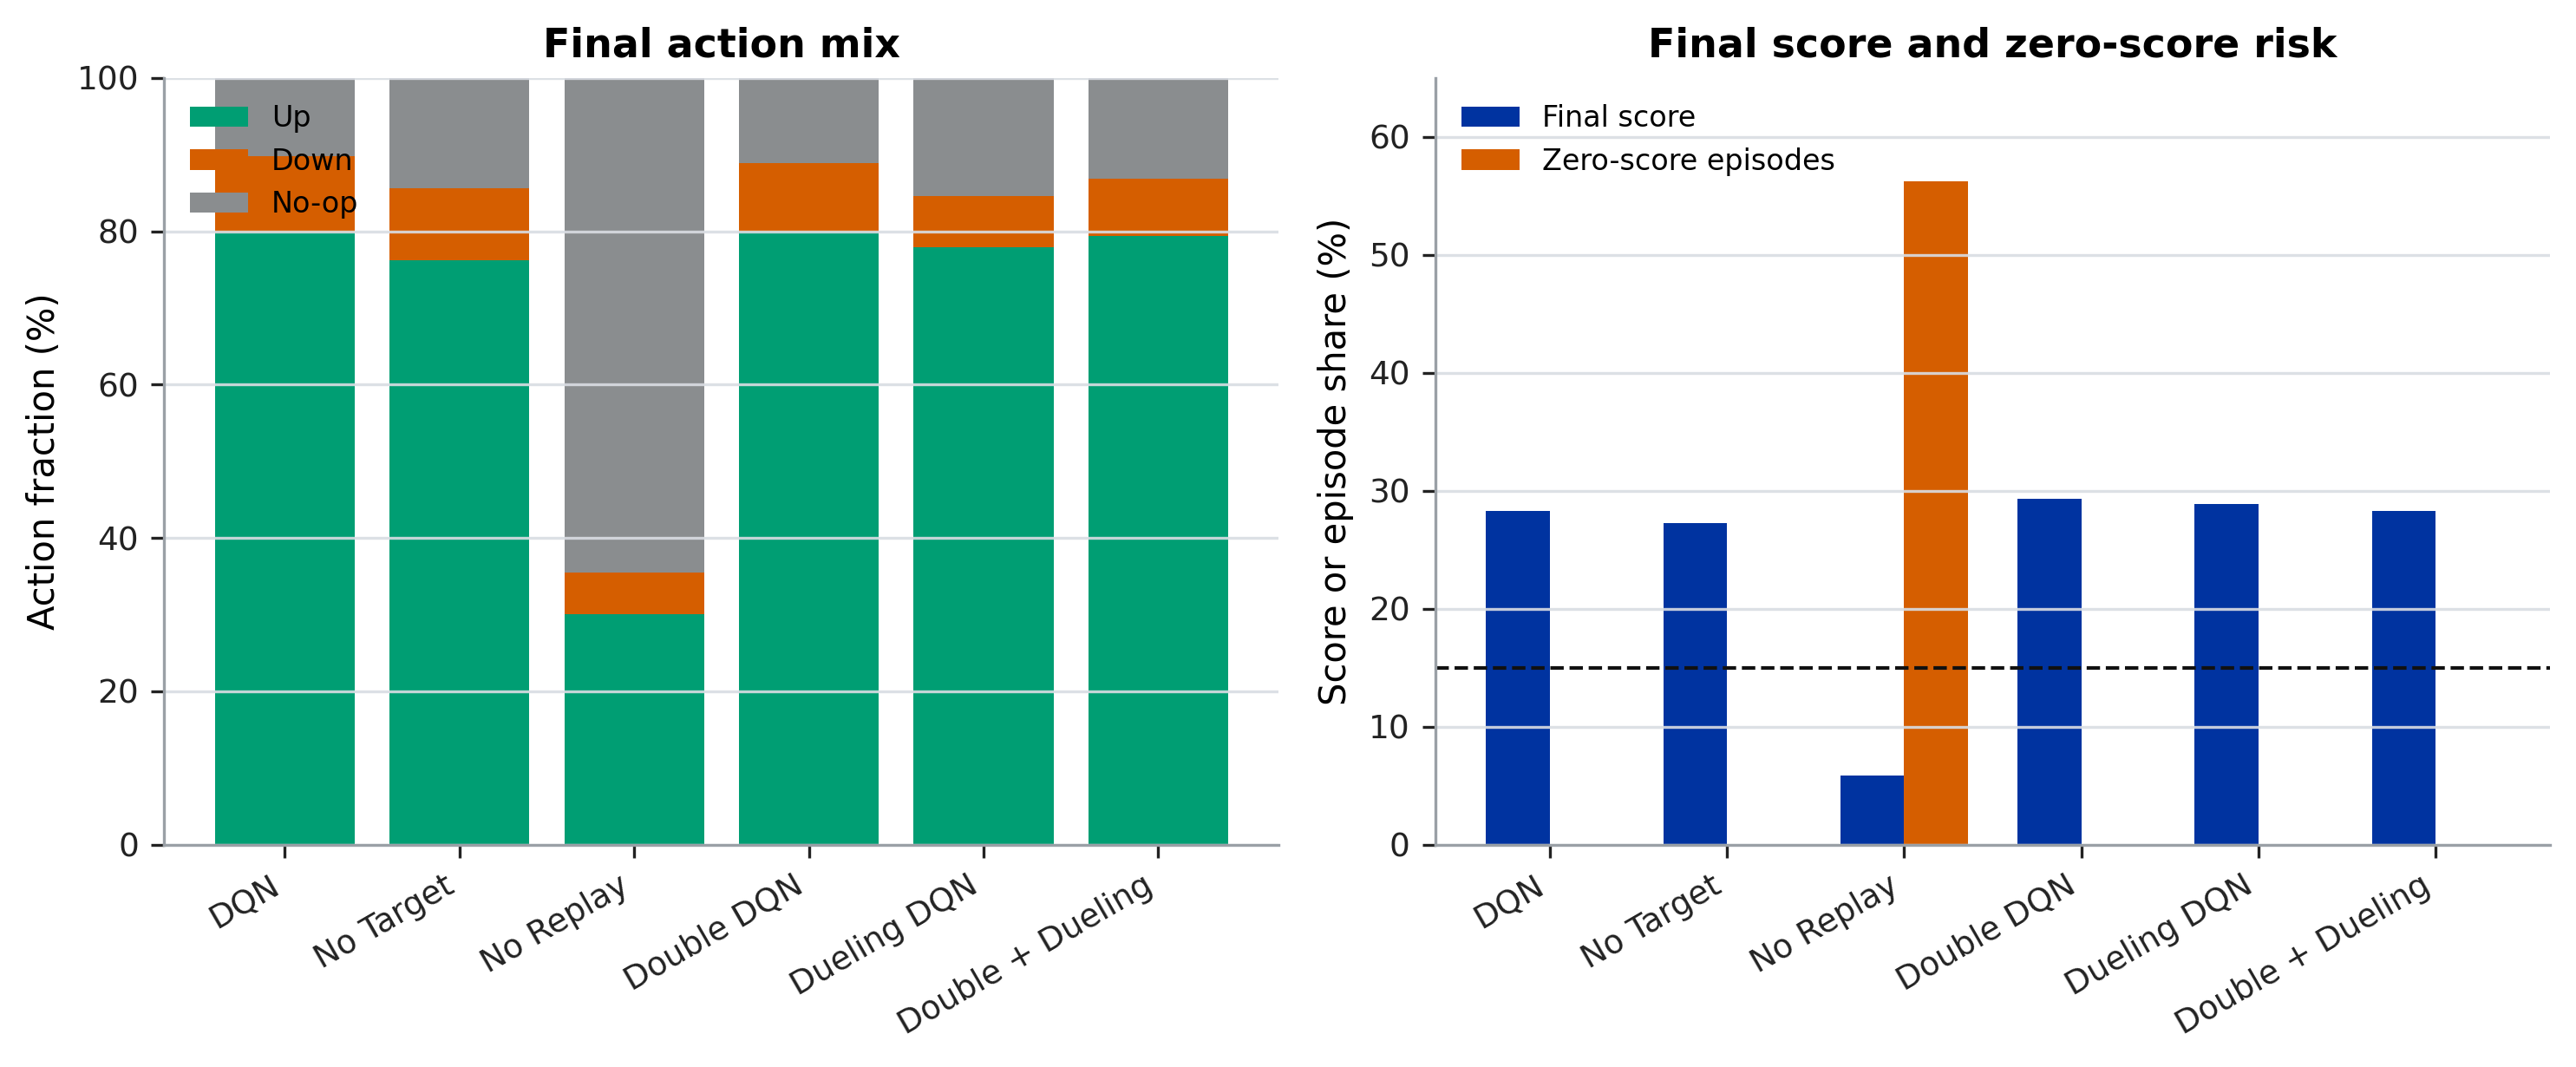
\includegraphics[width=0.9\linewidth]{helper/figures/freeway_final_behavior.png}
  \caption{Final Atari Freeway behavior. The left panel compares final action fractions, and the right panel compares final score with zero-score episode rate.}
  \label{fig:freeway-final-behavior}
\end{figure}

\subsubsection{Final Behavior}

Figure~\ref{fig:freeway-final-behavior} shows that the successful final policies have a simple action pattern. They mostly choose the upward action, with final up-action fractions between 76.2\% and 80.0\% for the replay-backed and no-target variants. This matches the task structure: the agent must keep moving upward while traffic interrupts progress.

The no-replay final policy looks different. Its final up-action fraction is only 30.0\%, while no-op actions take 64.5\% of its final behavior. It also has a 56.2\% final zero-score rate. This explains why its final return is much lower than its early threshold result. The failed policy is not only noisy; in most final episodes it stops making enough upward progress to score.

\subsubsection{Policy Retention}

The retention results are the clearest Freeway insight. The no-replay variant reaches score 15 in all four seeds, but it sustains score 15 in only one seed. It also reaches score 22.5 in only two seeds and has a mean peak-to-final gap of 15.7. This is a stronger version of the retention issue seen in Lunar Lander: finding a good policy once does not mean the agent will keep it.

The replay-backed variants show much better retention. DQN, Double DQN, Dueling DQN, and Double + Dueling DQN all reach and sustain score 15 in all four seeds, and all four variants reach score 22.5 in all four seeds. Double DQN has the smallest peak-to-final gap, 0.4, which matches its best final score. For Freeway, Double DQN is the best final-retention choice.

\begin{figure}[t]
  \centering
  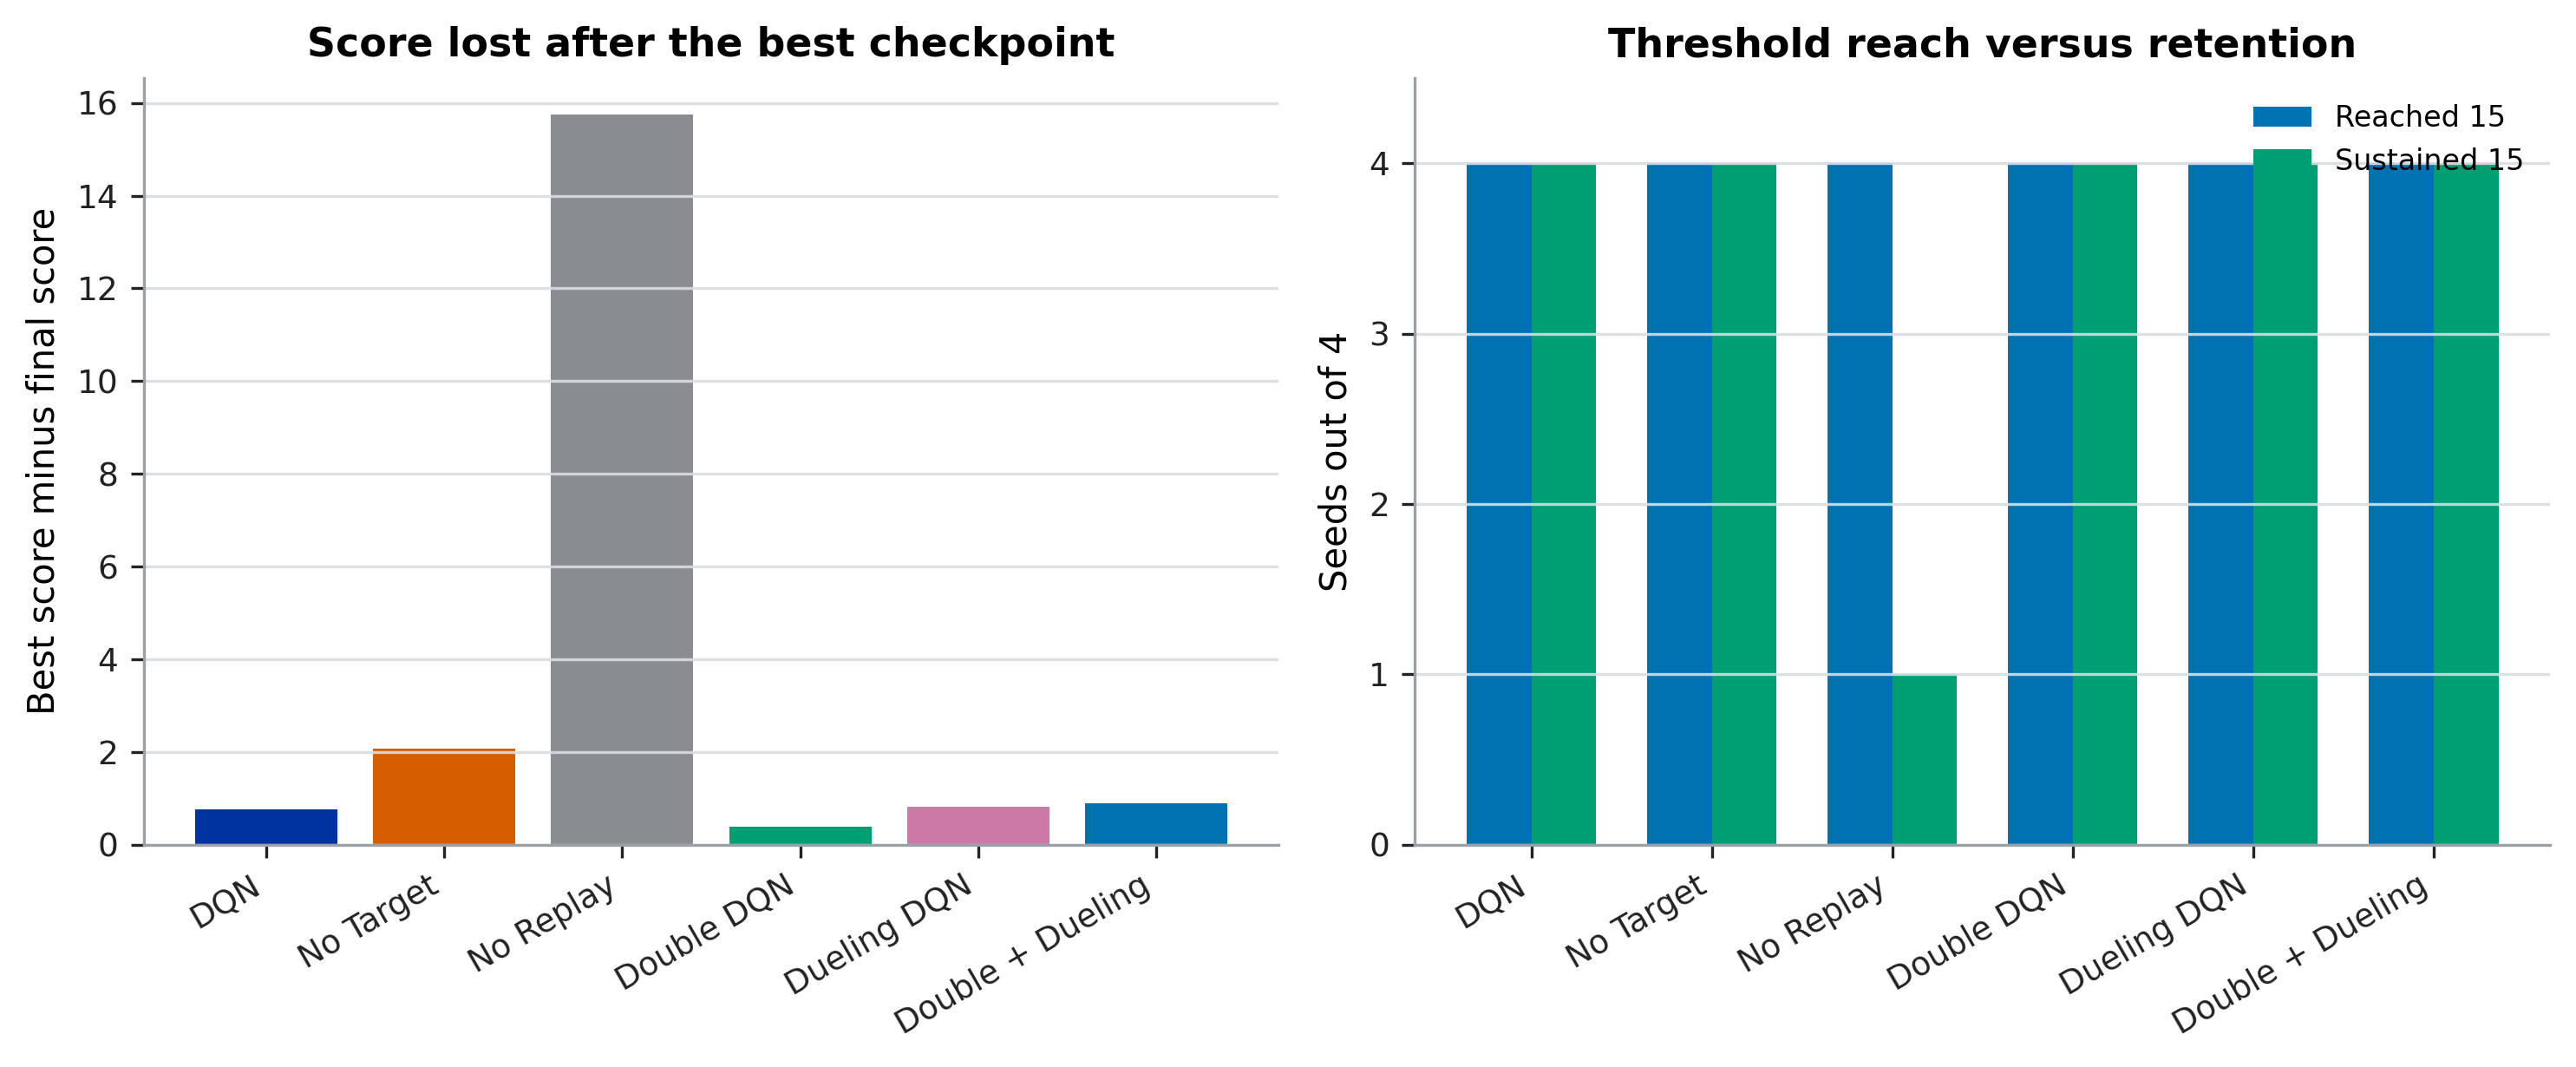
\includegraphics[width=0.87\linewidth]{helper/figures/freeway_retention_gap.png}
  \caption{Atari Freeway policy retention after learning. The left panel shows the average drop from each seed's best evaluation score to its final evaluation score. The right panel compares seeds that reached score 15 with seeds that sustained it.}
  \label{fig:freeway-retention}
\end{figure}

\subsubsection{Optimization Stress}

\begin{figure}[htbp]
  \centering
  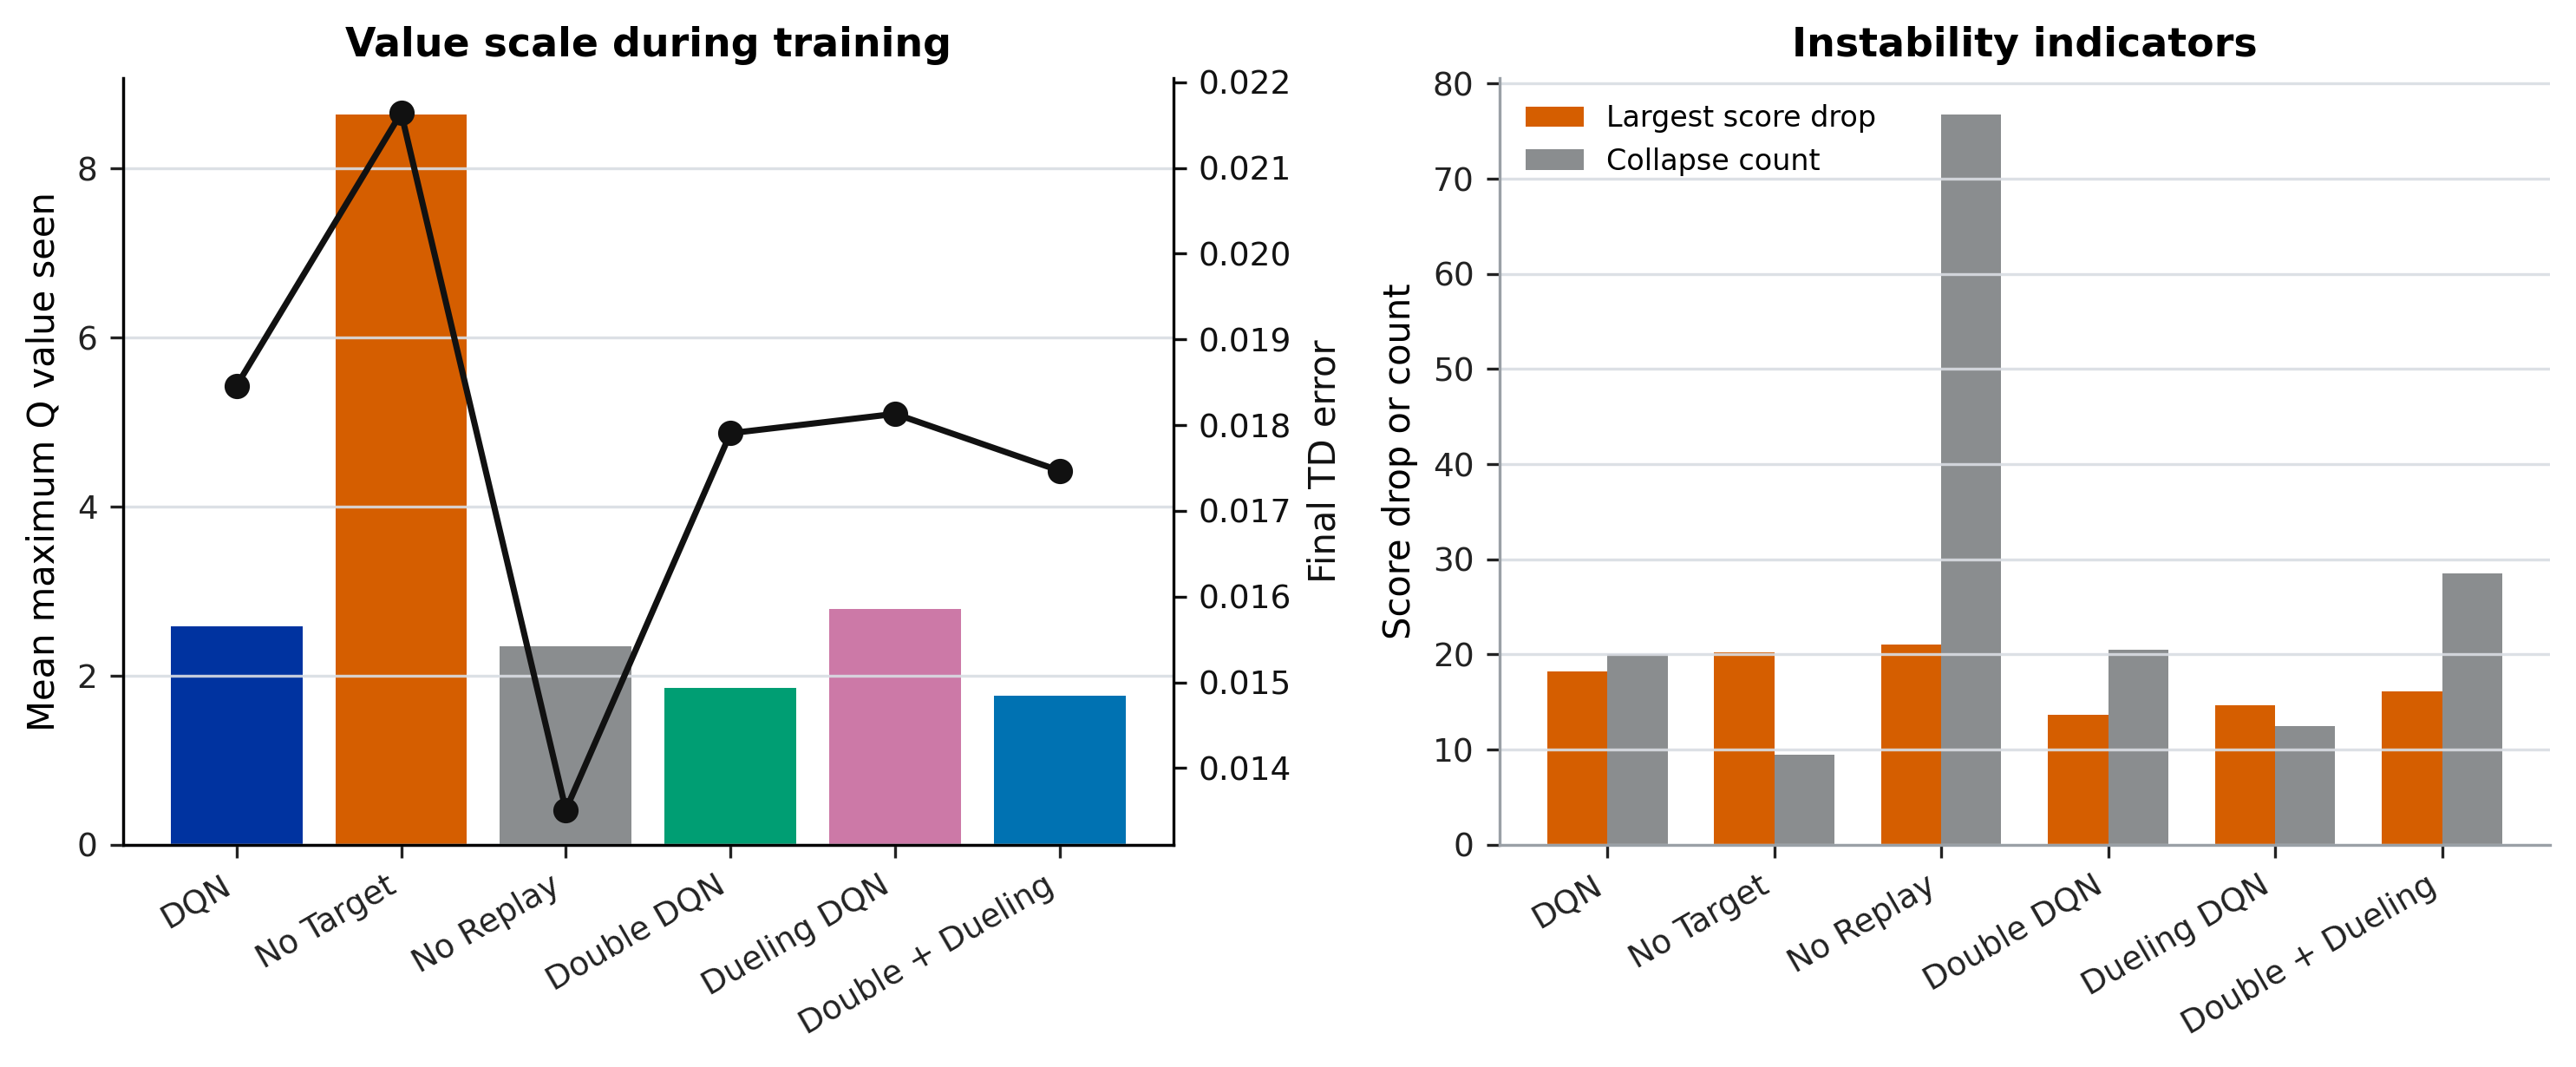
\includegraphics[width=0.87\linewidth]{helper/figures/freeway_optimization_stress.png}
  \caption{Optimization stress indicators for Atari Freeway. The value-scale panel overlays final TD error, and the instability panel compares largest score drop with average collapse count.}
  \label{fig:freeway-optimization-stress}
\end{figure}

Figure~\ref{fig:freeway-optimization-stress} shows that the target-network ablation has a different kind of stress from the replay ablation. The no-target variant has the largest value scale, with a mean maximum Q value of 8.64, while Double DQN and Double + Dueling DQN stay much lower at 1.86 and 1.76. The no-target variant also has the largest final TD error among the high-scoring variants. This supports the same idea as in Lunar Lander: the target network is important for keeping value estimates controlled.

The no-replay variant does not fail through a large Q-value scale. Its mean maximum Q value is 2.35 and its final TD error is small, but it has the highest mean collapse count, 76.8, and the worst final score. This means the loss can look calm after the policy has already become poor. In sparse Freeway, replay is essential because the agent needs to keep useful crossing experience in the update stream instead of learning mainly from recent low-reward behavior.

Overall, Freeway confirms that replay is the most important stabilizer for this implementation. The no-replay agent can discover crossing behavior under this run setting, but it usually cannot keep it. The target network matters more for value-scale control and final quality than for first reaching the threshold. Among the complete variants, Double DQN gives the best final score and the strongest retention.

\subsection{Aggregate Analysis}

The two task sections show the same six variants from different angles. To compare them directly, Table~\ref{tab:aggregate-comparison} normalizes each final score by its task threshold: return 200 for Lunar Lander and score 15 for Freeway. A value above 1.0 means the final policy is above the task reference. The same table also compares sustained-threshold rates and the normalized gap between the best checkpoint and the final checkpoint.

\begin{table}[htbp]
  \centering
  \caption{Cross-task comparison using task-threshold-normalized performance and retention.}
  \label{tab:aggregate-comparison}
  \scriptsize
  \begin{adjustbox}{width=\textwidth}
\begin{tabular}{@{}lccccccc@{}}
\toprule
\textbf{Variant} & \textbf{Lunar Final/Thr.} & \textbf{Freeway Final/Thr.} & \textbf{Mean Final/Thr.} & \textbf{Lunar Sustained} & \textbf{Freeway Sustained} & \textbf{Mean Sustained} & \textbf{Mean Peak Gap/Thr.} \\
\midrule
DQN & 1.04 & 1.89 & 1.46 & 70.0\% & 100.0\% & 85.0\% & 0.16 \\
No Target & 0.75 & 1.82 & 1.28 & 0.0\% & 100.0\% & 50.0\% & 0.35 \\
No Replay & -1.30 & 0.39 & -0.46 & 0.0\% & 25.0\% & 12.5\% & 1.50 \\
Double DQN & 1.10 & 1.96 & 1.53 & 50.0\% & 100.0\% & 75.0\% & 0.13 \\
Dueling DQN & 1.03 & 1.92 & 1.48 & 60.0\% & 100.0\% & 80.0\% & 0.18 \\
Double + Dueling & 1.10 & 1.89 & 1.49 & 90.0\% & 100.0\% & 95.0\% & 0.13 \\
\bottomrule
\end{tabular}
\end{adjustbox}

\end{table}

\begin{figure}[htbp]
  \centering
  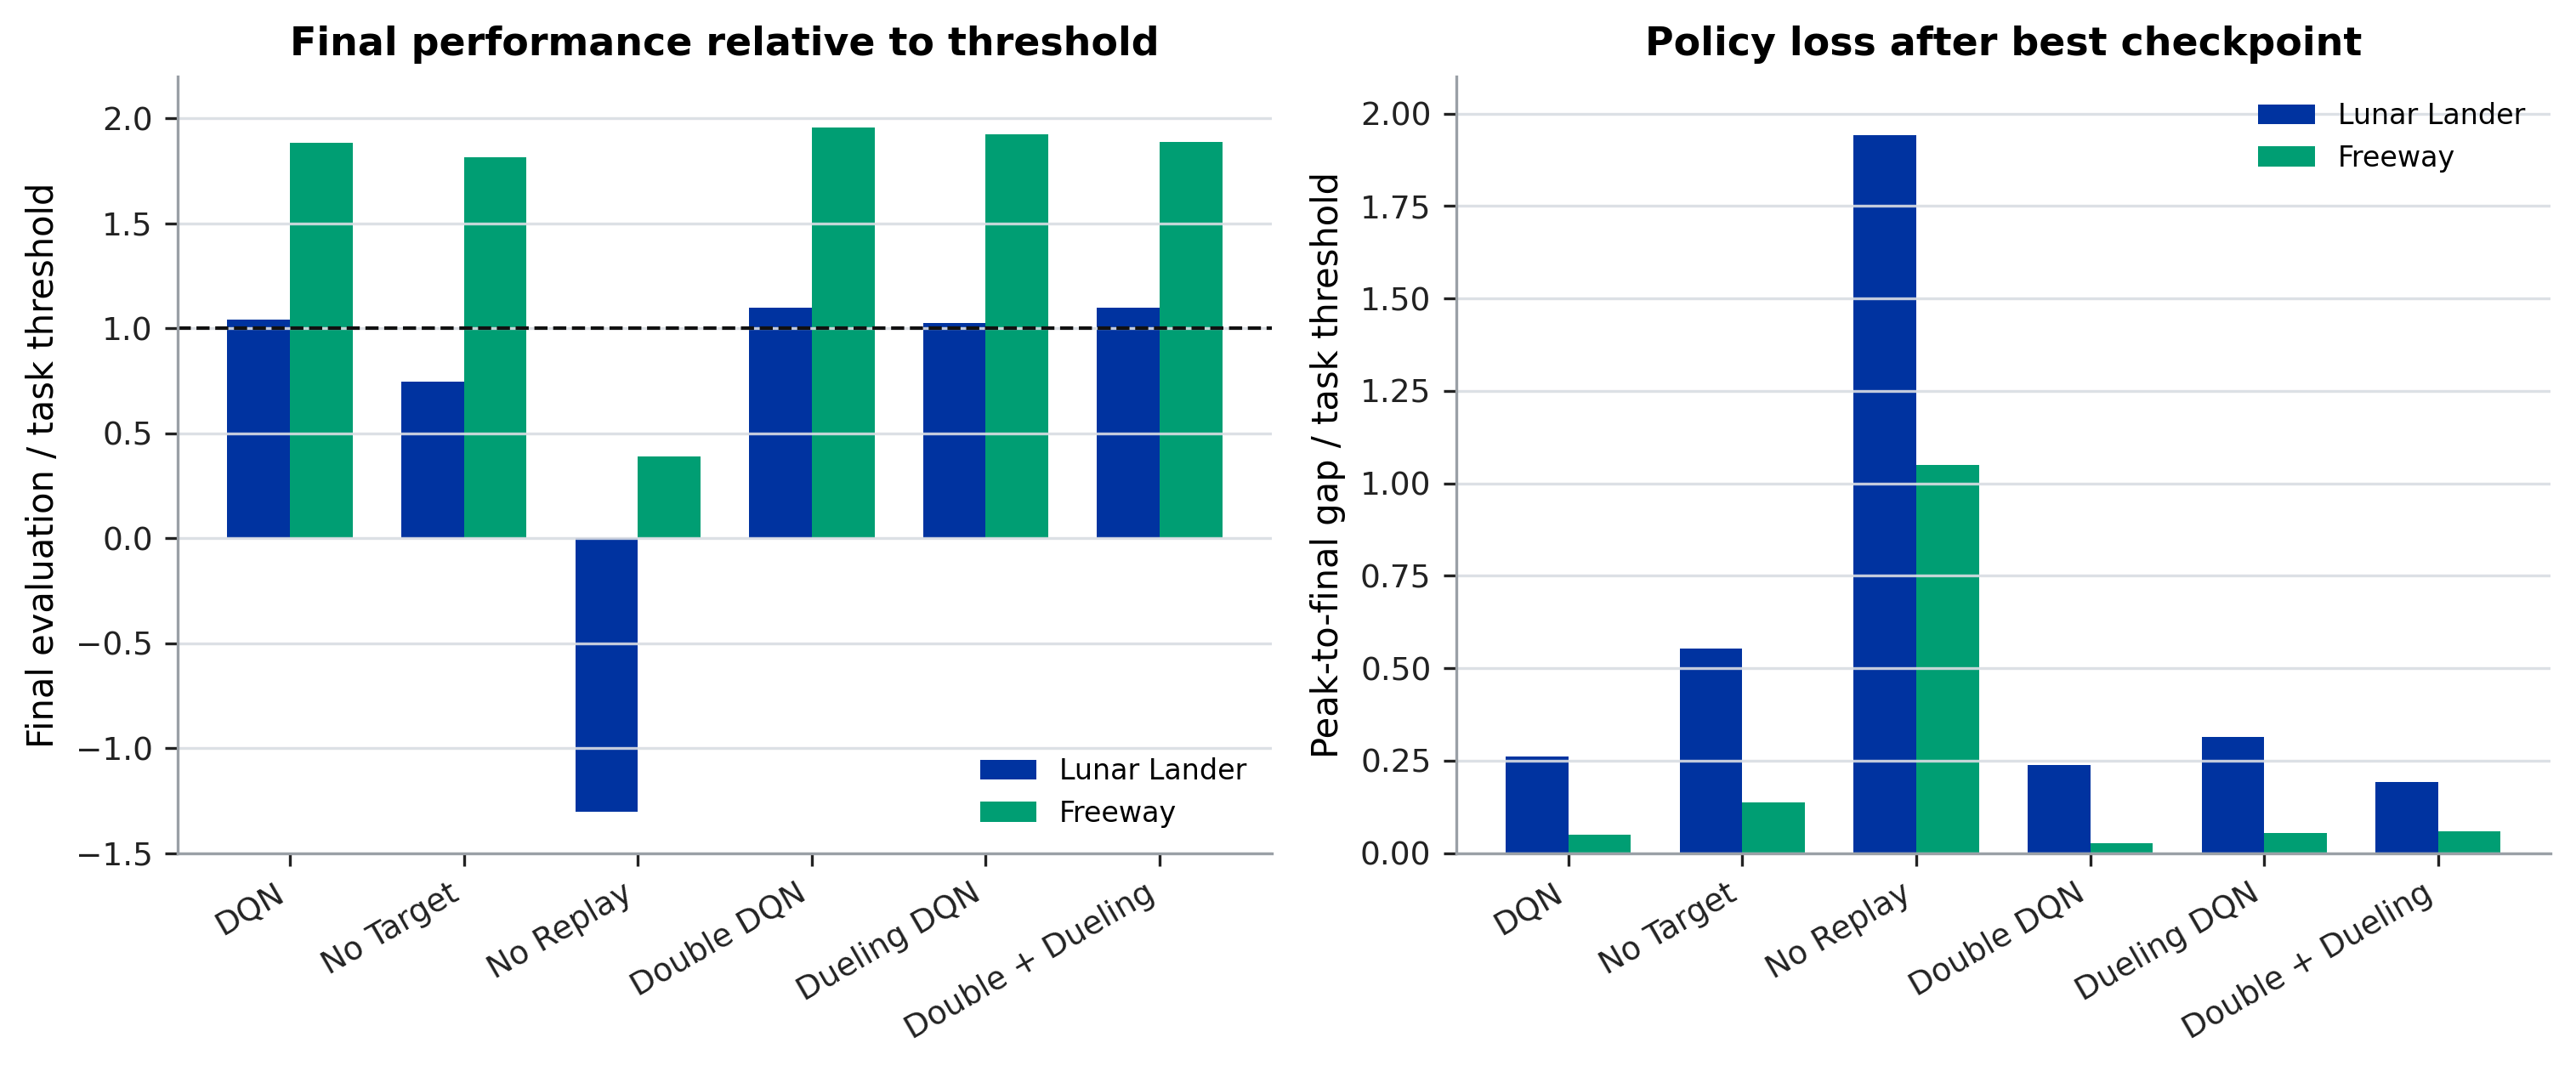
\includegraphics[width=0.87\linewidth]{helper/figures/aggregate_cross_task_stability.png}
  \caption{Cross-task aggregate stability. The left panel compares final performance divided by each task threshold. The right panel compares how much performance was lost from the best checkpoint to the final checkpoint, again divided by the task threshold.}
  \label{fig:aggregate-cross-task-stability}
\end{figure}

% The first cross-task insight is that reaching a threshold early is a weak signal when it is separated from retention. This was visible in each task alone, but the aggregate view makes the pattern stronger. The no-target variant reaches the main threshold in every seed for both tasks, yet its mean sustained rate across the two tasks is only 50.0\%. The no-replay variant is even weaker: it reaches score 15 in every Freeway seed and briefly reaches return 200 in one Lunar Lander seed, but its mean sustained rate is only 12.5\%. In both environments, a policy can find a useful behavior and still fail to keep it.

% The second cross-task insight is that the best variant depends on whether the goal is final score or retained success. Double DQN has the best mean final performance after threshold normalization, 1.53, because it combines a strong Lunar Lander final return with the best Freeway final score. Double + Dueling DQN is slightly lower on this final-performance average, 1.49, but it has the best mean sustained rate, 95.0\%, and nearly the same normalized peak-to-final gap. This makes Double DQN the best aggregate final-score choice, while Double + Dueling DQN is the better retention-oriented choice.

% Figure~\ref{fig:aggregate-cross-task-stability} also shows that the same ablation can fail with different visible symptoms across tasks. The no-replay variant finishes below the task threshold in both environments, and its peak-to-final loss is large in both tasks. The no-target variant is different: it stays above the Freeway threshold at the end, but it loses much more of its Lunar Lander peak. This supports the broader conclusion that replay is the more basic requirement for learning useful behavior, while the target network is most important for preserving stable value estimates after useful behavior appears.

The first cross-task insight is that early threshold crossing is a weak signal unless paired with retention. This pattern appears within each task, but becomes clearer in aggregate. The no-target variant reaches the main threshold in every seed for both tasks, yet its mean sustained rate across tasks is only 50.0\%. The no-replay variant is weaker: it reaches score 15 in every Freeway seed and briefly reaches return 200 in one Lunar Lander seed, but its mean sustained rate is only 12.5\%. In both environments, a policy can discover useful behavior without retaining it.

The second cross-task insight is that the best variant depends on whether the goal is final score or retained success. Double DQN has the best mean final performance after threshold normalization, 1.53, because it combines a strong Lunar Lander final return with the best Freeway final score. Double + Dueling DQN is slightly lower on this final-performance average, 1.49, but has the best mean sustained rate, 95.0\%, and nearly the same normalized peak-to-final gap. Thus, Double DQN is the best aggregate final-score choice, whereas Double + Dueling DQN is better for retention.

Figure~\ref{fig:aggregate-cross-task-stability} further shows that the same ablation can fail with different symptoms across tasks. The no-replay variant finishes below the task threshold in both environments and has large peak-to-final loss in both. The no-target variant differs: it remains above the Freeway threshold at the end, but loses much more of its Lunar Lander peak. This supports the broader conclusion that replay is the more basic requirement for learning useful behavior, while the target network is most important for preserving stable value estimates after useful behavior emerges.

\clearpage
\appendix
\section{Appendix}
\subsection{Project Source Bundle}

This appendix lists the source code used for this project.

\lstinputlisting[
  style=appendixcode,
  caption={Source code bundle generated by \texttt{gitingest} for this project.},
  label={lst:source}
]{source_code.txt}

\clearpage

\subsection{References}

\begingroup
\renewcommand{\section}[2]{}
\bibliographystyle{IEEEtran}
\bibliography{references}
\endgroup

\end{document}
